%!TEX encoding = UTF-8 Unicode
%!TEX root = ../exercises.tex

\ifPreSolution


\Exercise{\ExeWeekSEVEN}\label{exe:W07}

\begin{Goals}
%!TEX encoding = UTF-8 Unicode
%!TEX root = ../compendium2.tex

\item Kunna skapa och använda tupler, som variabelvärden, parametrar och returvärden.

\item Förstå skillnaden mellan ett objekt och en klass och kunna förklara betydelsen av begreppet instans.

\item Kunna skapa och använda attribut som medlemmar i objekt och klasser och som som klassparametrar.

\item Beskriva innebörden av och syftet med att ett attribut är privat.

\item Kunna byta ut implementationen av metoden \code{toString}.

\item Kunna skapa och använda en objektfabrik med metoden \code{apply}.

\item Kunna skapa och använda en enkel case-klass.

\item Kunna använda operatornotation och förklara relationen till punktnotation.

\item Förstå konsekvensen av uppdatering av föränderlig data i samband med multipla referenser.

\item Känna till och kunna använda några grundläggande metoder på samlingar.

\item Känna till den principiella skillnaden mellan \code{List} och \code{Vector}.

\item Kunna skapa och använda en oföränderlig mängd med klassen \code{Set}.

\item Förstå skillnaden mellan en mängd och en sekvens.

\item Kunna skapa och använda en nyckel-värde-tabell, \code{Map}.

\item Förstå likheter och skillnader mellan en \code{Map} och en \code{Vector}.

\end{Goals}

\begin{Preparations}
\item \StudyTheory{07}
\end{Preparations}

\else

\ExerciseSolution{\ExeWeekSEVEN}

\fi



\BasicTasks %%%%%%%%%%%%%%%%




\WHAT{Para ihop begrepp med beskrivning.}

\QUESTBEGIN

\Task \what

\vspace{1em}\noindent Koppla varje begrepp med den (förenklade) beskrivning som passar bäst:

\begin{ConceptConnections}
  linjärsökning & 1 & & A & avkoda symbolsekvens och återskapa objekt i minnet \\ 
  tidskomplexitet & 2 & & B & hur exekveringstiden växer med problemstorleken \\ 
  minneskomplexitet & 3 & & C & egenskapen att finnas kvar efter programmets avslut \\ 
  mängd & 4 & & D & unika identifierare, associerade med ett enda värde \\ 
  nyckel-värde-tabell & 5 & & E & unika element, kan snabbt se om element finns \\ 
  nyckelmängd & 6 & & F & leta i sekvens tills sökkriteriet är uppfyllt \\ 
  persistens & 7 & & G & för att snabbt hitta tillhörande värde \\ 
  serialisera & 8 & & H & hur minnesåtgången växer med problemstorleken \\ 
  de-serialisera & 9 & & I & koda objekt till avkodningsbar sekvens av symboler \\ 
\end{ConceptConnections}

\SOLUTION

\TaskSolved \what

\begin{ConceptConnections}
  mängd & 1 & ~~\Large$\leadsto$~~ &  F & unika element, kan snabbt se om element finns \\ 
  nyckel-värde-tabell & 2 & ~~\Large$\leadsto$~~ &  D & för att snabbt hitta tillhörande värde \\ 
  nyckelmängd & 3 & ~~\Large$\leadsto$~~ &  B & unika identifierare, associerade med ett enda värde \\ 
  persistens & 4 & ~~\Large$\leadsto$~~ &  C & egenskapen att finnas kvar efter programmets avslut \\ 
  serialisera & 5 & ~~\Large$\leadsto$~~ &  E & koda objekt till avkodningsbar sekvens av symboler \\ 
  de-serialisera & 6 & ~~\Large$\leadsto$~~ &  A & avkoda symbolsekvens och återskapa objekt i minnet \\ 
\end{ConceptConnections}

\QUESTEND


\WHAT{Typer i hierarkin av sekvenssamlingar.}

\QUESTBEGIN

\Task \what~Koppla varje typ i hierarkin av sekvenssamling med den (förenklade) beskrivning som passar bäst:

\begin{ConceptConnections}
  Traversable & 1 & & A & bastyp för alla sekvenssamlingar, indexposition från 0 \\ 
  Iterable & 2 & & B & bastyp för alla samlingar, har metoden \code|foreach| \\ 
  Seq & 3 & & C & är traverserbar med hjälp av metoden \code|iterator| \\ 
\end{ConceptConnections}

\SOLUTION

\TaskSolved \what

\begin{ConceptConnections}
  Traversable & 1 & ~~\Large$\leadsto$~~ &  A & bastyp för alla samlingar, har metoden \code|foreach| \\ 
  Iterable & 2 & ~~\Large$\leadsto$~~ &  C & är traverserbar med hjälp av metoden \code|iterator| \\ 
  Seq & 3 & ~~\Large$\leadsto$~~ &  B & bastyp för alla sekvenssamlingar, indexposition från 0 \\ 
\end{ConceptConnections}

\QUESTEND



\WHAT{Vad är en mängd?}
\QUESTBEGIN

\Task \what~ Förklara vad som händer nedan. Varför hamnar elementen i en ''konstig'' ordning? Varför ''försvinner'' det element?

\begin{REPL}
scala> val xs = Vector(1,2,3,1,2,3,4,5,7).toSet
xs: scala.collection.immutable.Set[Int] = Set(5, 1, 2, 7, 3, 4)
scala> xs.foreach(print)
512734
\end{REPL}

\SOLUTION

\TaskSolved \what~En mängd är en samling som snabbt kan ge svaret på frågan om ett visst element ingår i samlingen eller ej. Elementen i en mängd är unika. Tilläg av redan existerande element ignoreras. En mängd är inte en  sekvens, eftersom traversering med t.ex. \code{map} eller \code{foreach} inte (nödvändigtvis) sker i den ordning som elementen gavs när mängden konstruerades eller uppdaterades.

\QUESTEND


\WHAT{Använda mängder.}

\QUESTBEGIN

\Task \what

\vspace{1em}\noindent Para ihop varje uttryck till vänster med ett uttryck till höger som har samma värde:

\begin{ConceptConnections}
  \code|Set(1, 2) ++ Set(1, 2)          | & 1 & & A & \code|Set(1) + 2 + 3| \\ 
  \code|(1 to 3).toSet                  | & 2 & & B & \code|true          | \\ 
  \code|Vector.fill(3)(1).toSet         | & 3 & & C & \code|6             | \\ 
  \code|Set(1, 2, 3) diff Set(1, 2)     | & 4 & & D & \code|error: ...    | \\ 
  \code|(1 to 7).toSet.apply(8)         | & 5 & & E & \code|false         | \\ 
  \code|Set(1, 2, 3).sorted             | & 6 & & F & \code|Set(1, 2) - 2 | \\ 
  \code|Set(2,4) subsetOf (1 to 7).toSet| & 7 & & G & \code|Set(3)        | \\ 
  \code|Set(1, -1, 2, -2).map(_.abs).sum| & 8 & & H & \code|Set(1, 2)     | \\ 
  \code|Set(1, 1, 1, 1, 1, 5).sum       | & 9 & & I & \code|3             | \\ 
\end{ConceptConnections}

\SOLUTION

\TaskSolved \what

\begin{ConceptConnections}
  \code|Set(1, 2) ++ Set(1, 2)          | & 1 & ~~\Large$\leadsto$~~ &  H & \code|Set(1, 2)     | \\ 
  \code|(1 to 3).toSet                  | & 2 & ~~\Large$\leadsto$~~ &  G & \code|Set(1) + 2 + 3| \\ 
  \code|Vector.fill(3)(1).toSet         | & 3 & ~~\Large$\leadsto$~~ &  I & \code|Set(1, 2) - 2 | \\ 
  \code|Set(1, 2, 3) diff Set(1, 2)     | & 4 & ~~\Large$\leadsto$~~ &  D & \code|Set(3)        | \\ 
  \code|(1 to 7).toSet.apply(8)         | & 5 & ~~\Large$\leadsto$~~ &  B & \code|false         | \\ 
  \code|Set(1, 2, 3).sorted             | & 6 & ~~\Large$\leadsto$~~ &  C & \code|error: ...    | \\ 
  \code|Set(2,4) subsetOf (1 to 7).toSet| & 7 & ~~\Large$\leadsto$~~ &  A & \code|true          | \\ 
  \code|Set(1, -1, 2, -2).map(_.abs).sum| & 8 & ~~\Large$\leadsto$~~ &  F & \code|3             | \\ 
  \code|Set(1, 1, 1, 1, 1, 5).sum       | & 9 & ~~\Large$\leadsto$~~ &  E & \code|6             | \\ 
\end{ConceptConnections}

\QUESTEND


\WHAT{Räkna unika ord med hjälp av en mängd.}

\QUESTBEGIN

\Task \what~På veckans laboration ska vi göra automatisk språkbehandling av långa texter som vi delar upp i ord. Med metoden \code{s.split(' ').toVector} kan du dela upp en sträng \code{s} i en sekvens av ord, där \code{s} blivit uppdelad i många strängar vid varje blanktecken och alla blanktecken är borttagna.

\Subtask Använd metoderna \code{split} och \code{toSet} för skapa ett uttryck som beräknar hur många unika ord det finns i strängen \code{hej} nedan:
\begin{REPLnonum}
scala> val hej = "hej hej hemskt mycket hej"
\end{REPLnonum}

\Subtask Mängder är snabba på att kolla om ett element finns i mängden men du kan inte förvänta dig att elementen finns i någon viss ordning. Det finns en sekvenssamlingsmetod som skapar en sekvens med unika element ur en sekvens och behåller den ursprungliga ordningen. Vad heter metoden? \\\emph{Tips:} Leta i snabbreferensen eller sök på nätet. Metoden fungerar på alla samlingar som är av typen \code{Seq} och har ett namn som börjar med bokstäverna \code{di}.

\SOLUTION

\TaskSolved \what~

\SubtaskSolved
\begin{REPL}
scala> val hej = "hej hej hemskt mycket hej"
scala> val n = hej.split(' ').toSet.size
n: Int = 3
\end{REPL}

\SubtaskSolved Metoden \code{distinct} returnerar en sekvens med unika element och bibehållen ursprunglig ordning.

\QUESTEND




\WHAT{Skapa 2-tupler med metoden \code{->} som kan uttalas ''mappas till''.}

\QUESTBEGIN

\Task \what~Vi har tidigare sett hur två olika värden kan samlas i en 2-tupel, till exempel \code{(0, true)}. Par kan även skapas med hjälp av metoden \code{->} enligt nedan. Testa detta i REPL:
\begin{REPL}
scala> ("Skåne", "Lund")          // ett strängpar med vanlig 2-tupel
scala> "Skåne -> "Lund"           // operatornotation med ->
scala> "Skåne".->("Lund")         // punktnotation med -> (inte alls vanligt)
\end{REPL}
Metoden \code{->} fungerar med alla typer och är en fabriksmetod för par. Metodnamnet liknar en högerpil och illustrerar en mappning från första till andra värdet.

\Subtask Fungerar det på par skapade med \code{->} att använda metoderna \code{_1} och \code{_2}?


\Subtask Deklarera en variabel \code{val huvudstad: Vector[(String, String)]} som innehåller mappningar mellan geografiska områden och deras huvudstäder enligt tabellen nedan.

\begin{table}[H]
  \renewcommand{\arraystretch}{1.2}
  \begin{tabular}{|l|l|}\hline
  Sverige & Stockholm \\\hline
  Danmark & Köpenhamn \\\hline
  Grönland & Nuuk \\\hline
  Skåne & Lund \\\hline
  \end{tabular}
\end{table}

\Subtask Vad blir det för felmeddelande om du råkar skriva ett komma för mycket före den avslutande högerparentesen: ...\code{und",)}

\Subtask Skriv ett uttryck som plockar fram \code{"Lund"} ur \code{huvudstad}.

\SOLUTION


\TaskSolved \what

\SubtaskSolved Ja, fabriksmetoden returnerar ett helt vanligt par:
\begin{REPLnonum}
scala> val härBorJag = "Skåne" -> "Lund"
härBorJag: (String, String) = (Skåne,Lund)

scala> härBorJag._1
res0: String = Skåne

scala> härBorJag._2
res1: String = Lund
\end{REPLnonum}


\SubtaskSolved

\begin{Code}
val huvudstad = Vector(
  "Sverige"  -> "Stockholm",
  "Danmark"  -> "Köpenhamn",
  "Grönland" -> "Nuuk",
  "Skåne"    -> "Lund"
)
\end{Code}

\SubtaskSolved

\begin{REPL}
scala> Vector("Sverige"->"Stockholm","Norge"->"Oslo","Skåne"->"Lund",)
<console>:1: error: illegal start of simple expression
\end{REPL}
Man skriver ofta en mappning per rad för att det ska gå att läsa som en tabell, och inte som ovan med alla mappningar på samma rad.

Det är lätt hänt att få med ett komma för mycket (eller för lite) när man flyttar eller duplicerar rader med många mappningar i en kodeditor. I en framtida version av Scala kommer sådana problem att vara mindre smärtsamma:\\
\url{http://docs.scala-lang.org/sips/completed/trailing-commas.html}

\SubtaskSolved
\begin{REPL}
scala> huvudstad(2)._2
res2: String = Lund
\end{REPL}

\QUESTEND



\WHAT{Linjärsöka efter nyckel i sekvens av mappningar.}

\QUESTBEGIN

\Task \what~

\Subtask Implementera funktionen \code{lookupIndex} nedan med hjälp av samlingsmetoden \code{indexWhere} så att linjärsökning sker efter index för ett par i sekvensen där \code{key} finns på första platsen i paret.

\begin{Code}
def lookupIndex(xs: Vector[(String, String)])(key: String): Int = ???
\end{Code}

\Subtask Testa din funktion i REPL genom att slå upp index för Skånes huvudstad i sekvensen \code{huvudstad} från föregående uppgift.

\SOLUTION

\TaskSolved \what~

\SubtaskSolved
\begin{Code}
def lookupIndex(xs: Vector[(String, String)])(key: String): Int =
  xs.indexWhere(_._1 == key)
\end{Code}

\SubtaskSolved
\begin{REPL}
scala> val i = lookupIndex(huvudstad)("Skåne")
i: Int = 3

scala> huvudstad(i)._2
res2: String = Lund
\end{REPL}

\noindent Eller med funktioner som återanvändbara dellösningar:
\begin{REPL}
scala> val indexOf = lookupIndex(huvudstad) _

scala> def capital(key: String) = huvudstad(indexOf(key))._2

scala> capital("Skåne")
res3: String = Lund

scala> capital("Sverige")
res4: String = Stockholm
\end{REPL}

\QUESTEND



\WHAT{Nyckel-värde-tabell.}

\QUESTBEGIN

\Task \what~En nyckel-värde-tabell är en smart datastruktur som gör att du kan slå upp det värde som en nyckel mappar till \emph{utan} att linjärsökning behöver ske. Värdet plockas fram direkt på en konstant tid, d.v.s. tiden att slå upp ett värde beror \emph{inte} på antalet element i samlingen, utan sker med mycket liten fördröjning.

I Scala heter nyckelvärdetabeller \code{Map} med stort M och är praktiska att använda i många olika sammanhang. \code{Map} finns i både en oföränderlig och en förändringsbar variant. Det går med metoder på formen \code{toXXX} lätt att omvandla mellan en \code{Map} och en sekvens av par av typen \code{XXX[(Nyckeltyp, Värdetyp)]}.

\Subtask Deklarera mappen \code{telnr} nedan i REPL och använd \code{apply} för att ta reda på telefonnumret till Fröken Ur.

\Subtask Vad har \code{telnr} för typ?

\Subtask Vad har \code{telnr.toVector} för typ?

\begin{Code}
val telnr = Map(
  "Anna"     -> 46462229812L,
  "Björn"     -> 46462229009L,
  "Sandra"    -> 46462220368L,
  "Fröken Ur" -> 4690510L,
)
\end{Code}
En uppsättning \code{Map}-instanser, vid behov nästlade, kan med fördel användas för att bygga upp en i-minnet-databas där inbyggda samlingsmetoder, t.ex. \code{map}, \code{filter}, och \code{for}-\code{yield}-uttryck, ger flexibla och effektiva sökmöjligheter. På veckans laboration ska du göra detta.

Samlingen \code{Map} är en generalisering av en sekvens, där man kan ''indexera'', inte bara med ett heltal, utan med vilken typ av värde som helst, t.ex. en sträng. Datastrukturen \code{Map} kallas också \emph{associativ array}\footnote{\href{https://en.wikipedia.org/wiki/Associative_array}{https://en.wikipedia.org/wiki/Associative\_array}} och är implementerad som en s.k. \emph{hashtabell}\footnote{\href{https://en.wikipedia.org/wiki/Hash_table}{https://en.wikipedia.org/wiki/Hash\_table}}, men du får vänta till fördjupningskursen innan vi går igenom hur en sådan datastruktur implementeras.

\SOLUTION

\TaskSolved \what~

\begin{REPL}
scala> telnr("Fröken Ur")
res0: Long = 464690510

scala> :type telnr
scala.collection.immutable.Map[String,Long]

scala> :type telnr.toVector
Vector[(String, Long)]
\end{REPL}

\QUESTEND



\WHAT{Använda nyckel-värdetabell.}

\QUESTBEGIN

\Task \what~

\Subtask Skapa nedan variabler i REPL.
\begin{Code}
val xs = (for (i <- 2 to 16 by 2) yield (i, i + 1)).toMap
val ys = xs.toVector
\end{Code}
Hamnar mappningarna i \code{ys} i samma ordning som de skapades med for-uttrycket?

\Subtask Med \code{xs} och \code{ys} deklarerade i REPL enligt ovan, para ihop yttryck till vänster med rätt resultat till höger. Om du är osäker på de sammansatta uttrycken, prova enklare uttryck i REPL och undersök värde och typ hos delresultat.

\begin{ConceptConnections}
  \code|xs(2) + xs(4)                 | & 1 & & A & \code|true                  | \\ 
  \code|ys(2) + ys(4)                 | & 2 & & B & \code|1                     | \\ 
  \code|ys(0)                         | & 3 & & C & \code|NoSuchElementException| \\ 
  \code|xs(0)                         | & 4 & & D & \code|(16, 17)              | \\ 
  \code|(xs + (0 -> 1)).apply(0)      | & 5 & & E & \code|-9                    | \\ 
  \code|xs.keySet.apply(2)            | & 6 & & F & \code|8                     | \\ 
  \code|xs.mapValues(v => -v).apply(8)| & 7 & & G & \verb|error: type mismatch  | \\ 
  \code|xs isDefinedAt 0              | & 8 & & H & \code|false                 | \\ 
  \code|xs.getOrElse(0, 7)            | & 9 & & I & \code|(10, 11)              | \\ 
  \code|xs.maxBy(_._2)                | & 10 & & J & \code|7                     | \\ 
\end{ConceptConnections}

\SOLUTION

\TaskSolved \what


\SubtaskSolved Nej nyckel-värde-paren lagras i någon speciell ordning som bestäms av en intern, smart lagringsprincip enligt en s.k. hashfunktion\footnote{\url{https://sv.wikipedia.org/wiki/Hashfunktion}}, för att åstadkomma snabba uppslagningar av värden från nycklar och vilket normalt inte sammanfaller med ordningen i den sekvens som de skapades ur.

\SubtaskSolved

\begin{ConceptConnections}
    \code|xs(2) + xs(4)                 | & 1 & ~~\Large$\leadsto$~~ &  E & \code|8                     | \\ 
  \code|ys(2) + ys(4)                 | & 2 & ~~\Large$\leadsto$~~ &  B & \verb|error: type mismatch  | \\ 
  \code|ys(0)                         | & 3 & ~~\Large$\leadsto$~~ &  I & \code|(10, 11)              | \\ 
  \code|xs(0)                         | & 4 & ~~\Large$\leadsto$~~ &  H & \code|NoSuchElementException| \\ 
  \code|(xs + (0 -> 1)).apply(0)      | & 5 & ~~\Large$\leadsto$~~ &  F & \code|1                     | \\ 
  \code|xs.keySet.apply(2)            | & 6 & ~~\Large$\leadsto$~~ &  G & \code|true                  | \\ 
  \code|xs.mapValues(v => -v).apply(8)| & 7 & ~~\Large$\leadsto$~~ &  C & \code|-9                    | \\ 
  \code|xs isDefinedAt 0              | & 8 & ~~\Large$\leadsto$~~ &  J & \code|false                 | \\ 
  \code|xs.getOrElse(0, 7)            | & 9 & ~~\Large$\leadsto$~~ &  D & \code|7                     | \\ 
  \code|xs.maxBy(_._2)                | & 10 & ~~\Large$\leadsto$~~ &  A & \code|(16, 17)              | \\ 
\end{ConceptConnections}

\noindent \emph{Fördjupning}:  Felmeddelandet som rad 2 ovan orsakar är lurigt:

\begin{REPL}
scala> ys(2)
res22: (Int, Int) = (6,7)

scala> ys(4)
res23: (Int, Int) = (12,13)

scala> ys(2) + ys(4)
<console>:13: error: type mismatch;
 found   : (Int, Int)
 required: String
       ys(2) + ys(4)

\end{REPL}
Det går som förväntat inte att addera två tupler, men varför säger kompilatorn att en sträng krävs?!? Detta beror på att, i enlighet med hur det fungerar i Java, valde Scala-språkets konstruktörer att låta strängsammanfogning fungera med alla möjliga typer vilket gör att kompilatorn inte ger upp när metoden \code{+} inte finns för tupler, utan i stället gör ett misslyckat försök med strängsammanfogning.

Det mest olyckliga med detta är inte att felmeddelanden ibland blir missvisande, utan att det i vissa situationer inte ens \emph{blir} något felmeddelande, trots att man av rent misstag råkat strängkonkatenera i stället för t.ex. lägga till ett element i en mängd eller en mappning i en tabell. Detta typosäkra beteendet av strängsammanfogning har kritiserats, men det är inte okontroversiellt att ändra detta nu när så många utvecklare skrivit så mycket Scala-kod som bygger på strängars förmåga att kunna lägga till vad som helst på slutet. Situationen i Scala är dock inte hopplös efter introduktionen av stränginterpolering i Scala 2.10, som möjliggör infogande av värden i strängar på ett typsäkert sätt.
\QUESTEND





\WHAT{Registrering i förändringsbar nyckel-värde-tabell.}

\QUESTBEGIN

\Task \what~I denna uppgift ska du implementera en hjälpklass för registrering i en frekvenstabell som du sedan ska använda på veckans laboration. Klassen ska heta  \code{FreqMapBuilder} som efter upprepade anrop av metoden \code{add(s: String): Unit} kan skapa frekvenstabeller av typen \code{Map[String, Int]}, där nyckel-värde-paren i tabellen anger antalet förekomster av en viss sträng. Du ska utgå från koden nedan.

Klassen använder en förändringsbar tabell internt. Efter att man har lagt till många strängar kan man med metoden \code{toMap} få en oföränderlig tabell för  uppslagning av frekvenser för specifika strängar. Läs i snabbreferensen om vilka extra metoder för uppdatering som erbjuds av \code{mutable.Map[K, V]}.

\begin{Code}
class FreqMapBuilder {
  private val register = collection.mutable.Map.empty[String, Int]
  def toMap: Map[String, Int] = register.toMap
  def add(s: String): Unit = ???
}
object FreqMapBuilder {
  def apply(xs: String*): FreqMapBuilder = ???
}
\end{Code}

\noindent Implementera och testa \code{FreqMapBuilder}. \emph{Tips:} Du kan t.ex. använda metoderna \code{+=} och \code{getOrElse}.

\SOLUTION

\TaskSolved \what~
\begin{Code}
class FreqMapBuilder {
  private val register = scala.collection.mutable.Map.empty[String,Int]
  def toMap: Map[String, Int] = register.toMap
  def add(s: String): Unit =
    register += (s -> (register.getOrElse(s, 0) + 1))
}
object FreqMapBuilder {
  def apply(xs: String*): FreqMapBuilder = {
    val result = new FreqMapBuilder
    xs.foreach(result.add)
    result
  }
}
\end{Code}

\QUESTEND



\WHAT{Metoden \code{sliding}.}

\QUESTBEGIN

\Task  \what~  I veckans laboration kommer du att ha nytta av metoden \code{sliding}, som ger en iterator för speciella delsekvenser av en sekvens, vilka kan liknas vid ''utsikten'' i ett ''glidande fönster''.

\Subtask Kör nedan i REPL och beskriv vad som händer.

\begin{REPL}
scala> val xs = Vector("fem", "gurkor", "är", "fler", "än", "fyra", "tomater")
scala> xs.sliding(2).toVector
scala> xs.sliding(3).toVector
scala> xs.sliding(10).toVector
\end{REPL}

\Subtask Använd \code{xs.sliding(2)} och omvandla varje element i resultatet till ett par. Gör sedan om sekvensen av par till en nyckel-värde-tabell. Vad kan tabellen användas till?

\SOLUTION

\TaskSolved \what

\SubtaskSolved
\begin{REPL}
scala> val xs = Vector("fem", "gurkor", "är", "fler", "än", "fyra", "tomater")
xs: scala.collection.immutable.Vector[String] =
Vector(fem, gurkor, är, fler, än, fyra, tomater)

scala> xs.sliding(2).toVector
res9: Vector[scala.collection.immutable.Vector[String]] =
Vector(Vector(fem, gurkor), Vector(gurkor, är), Vector(är, fler), Vector(fler, än), Vector(än, fyra), Vector(fyra, tomater))

scala> xs.sliding(3).toVector
res10: Vector[scala.collection.immutable.Vector[String]] =
Vector(Vector(fem, gurkor, är), Vector(gurkor, är, fler), Vector(är, fler, än), Vector(fler, än, fyra), Vector(än, fyra, tomater))

scala> xs.sliding(10).toVector
res11: Vector[scala.collection.immutable.Vector[String]] =
Vector(Vector(fem, gurkor, är, fler, än, fyra, tomater))

\end{REPL}
\code{xs.sliding(n).toVector} skapar en sekvens som innehåller sekvenser av längden \code{n} som bildas genom att ta varje element och dess \code{n - 1} efterföljande element.

\SubtaskSolved
\begin{REPL}
scala> xs.sliding(2).map(ys => ys(0) -> ys(1)).toMap
res0: scala.collection.immutable.Map[String,String] =
Map(är -> fler,
    än -> fyra,
    fyra -> tomater,
    gurkor -> är,
    fem -> gurkor,
    fler -> än
)
\end{REPL}
Man kan använda tabellen till att slå upp vilket som är efterföljande ord. Det fungerar eftersom alla ord är unika. Om det funnits flera likadana ord med olika efterföljande ord så hade vi behövt skapa en tabell med nycklar som mappar till en samling som registrerar efterföljande ord. Detta ska vi göra på veckans laboration.

\QUESTEND




\WHAT{Läsa text från fil och webbservrar.}

\QUESTBEGIN

\Task \what~På laborationen ska du bygga upp tabeller från data i textformat. Då har du nytta av att kunna läsa text från filer och från webben. Testa detta i REPL:
\begin{REPL}
scala> val url = "https://fileadmin.cs.lth.se/pgk/europa.txt"
scala> val xs = io.Source.fromURL(url, "UTF-8").getLines.toVector
scala> val data = xs.map(_.split(';').toVector)
scala> data.head
scala> data.foreach(println)
\end{REPL}

\Subtask Skapa dessa tabeller ur sekvensen \code{data}:
\begin{Code}
val populationOf: Map[String, Int]    = ???  // länders invånarantal
val sizeOf:       Map[String, Int]    = ???  // länders yta i km^2
val capitalOf:    Map[String, String] = ???  // länders huvudstäder
\end{Code}
Testa tabellerna i REPL.

\Subtask Spara ner data i en textfil \code{europa.txt}. Läsa in data från filen med metoden \code{Source.fromFile(filnamn, teckenkodning)} på liknande sätt som med  \code{fromURL} ovan. Om du kör i en Linux-terminal kan du enkelt ladda ner en fil så här:
\begin{REPLnonum}
> wget https://fileadmin.cs.lth.se/pgk/europa.txt
\end{REPLnonum}
Skriv ut alla raderna i \code{europa.txt} med hjälp av \code{Source.fromFile} i REPL.

\SOLUTION

\TaskSolved \what~

\SubtaskSolved
\begin{CodeSmall}
val populationOf = data.tail.map(v => v(0) -> v(1).toInt).toMap
val sizeOf       = data.tail.map(v => v(0) -> v(2).toInt).toMap
val capitalOf    = data.tail.map(v => v(0) -> v(3)).toMap
\end{CodeSmall}

\begin{REPL}
scala> capitalOf("Sverige")
res2: String = Stockholm

scala> populationOf("Sverige")
res3: Int = 9223766

scala> sizeOf("Sverige")
res4: Int = 449964
\end{REPL}

\begin{REPL}
scala> val filename = "europa.txt"
scala> val xs = io.Source.fromFile(filename, "UTF-8").getLines.toVector
scala> val data = xs.map(_.split(';').toVector)
scala> data.map(_.map(_.take(15).padTo(15,' ')).mkString(" ")).foreach(println)
\end{REPL}
\QUESTEND





\ExtraTasks %%%%%%%%%%%%%%%%%%%%%%%%%%%%%%%%%%%%%%%%%%%%%%%%%%%%%%%%%%%%%%%%%%%%

\WHAT{Skapa ett textspel med hjälp av tabeller.}

\QUESTBEGIN

\Task \what~Gör ett enkelt spel för att träna på olika fakta om Europas länder och huvudstäder genom att läsa data från URL:en:\\ \url{https://fileadmin.cs.lth.se/pgk/europa.txt}
\\Där finns text kodad i UTF-8 med följande innehåll (endast de första raderna visas):
\begin{Code}
Land;Invånarantal;Storlek(km^2);Huvudstad
Albanien;3581655;28748;Tirana
Andorra;71201;468;Andorra la Vella
Belgien;10584534;30528;Bryssel
Bosnien-Hercegovina;4590310;51129;Sarajevo
Bulgarien;7385367;110910;Sofia
Cypern;854000;9250;Nicosia
Danmark;5475791;43094;Köpenhamn
Estland;1324333;45226;Tallinn
Finland;5315280;338145;Helsingfors
Frankrike;61538322;551695;Paris
Färöarna;48344;139574;Torshamn
Grekland;10964021;131940;Aten
// ... etcetera för alla Europas länder.
\end{Code}
Låt till exempel användaren svara på slumpvisa frågor av typen:
\begin{itemize}[noitemsep]
  \item Har Andorra fler invånare än Cypern?
  \item Vad heter huvudstaden i Bulgarien?
  \item Har Danmark större yta än Finland?
\end{itemize}
Använd oföränderliga tabeller med lämpliga nycklar och värden. Du kan använda en mängd med länder/huvudstäder som användaren hittills svarat rätt på för att kunna förhindra att dessa återkommer igen.
\SOLUTION

\TaskSolved --

\QUESTEND



\AdvancedTasks %%%%%%%%%%%%%%%%%%%%%%%%%%%%%%%%%%%%%%%%%%%%%%%%%%%%%%%%%%%%%%%%%


\WHAT{Registrering med \code{groupBy} och \code{mapValues}.}

\QUESTBEGIN

\Task \what~Vi ska nu utnyttja ett riktigt listigt trick för att via en enda kodrad implementera registrering med hjälp av samlingsmetoden \code{groupBy} och tabellmetoden \code{mapValues}.

\Subtask Läs om metoden \code{groupBy} i snabbreferensen. Du hittar den under rubriken \emph{''Methods in trait \code{Traversable[A]}''} eftersom \code{groupBy} fungerar på alla samlingar. Testa \code{groupBy} enligt nedan och beskriv vad som händer.

\begin{REPL}
scala> val xs = Vector(1, 1, 2, 2, 4, 4, 4).groupBy(x => x > 2)
scala> val ys = Vector(1, 1, 2, 2, 4, 4, 4).groupBy(x => x)
\end{REPL}

\Subtask Skapa en funktion \code{freq} med nedan funktionshuvud som returnerar en tabell med antalet förekomster av olika heltal i \code{xs}. Testa \code{freq} på en sekvens av 1000 slumpvisa tärningskast och förklara hur funktionen \code{freq} fungerar. \emph{Tips:} Gör först \code{groupBy(???)} och sedan \code{mapValues(???)}.

\begin{Code}
def freq(xs: Vector[Int]): Map[Int, Int] = ???

def kasta(n: Int): Vector[Int] =
  Vector.fill(n)(scala.util.Random.nextInt(6) + 1)
\end{Code}

\SOLUTION

\TaskSolved \what~

\SubtaskSolved Metoden \code{groupBy} skapar en nyckel-värde-tabell där värdena i tabellen är en sekvens med elementen grupperade på ett speciellt sett.
Mer precist:

Resultatet av \code{xs.groupBy(f: K => V)} för en sekvens \code{xs} av typen \code{Vector[K]} blir en tabell av typen \code{Map[V,Vector[K]]} där varje element \code{e} i \code{xs} är grupperade i samma tabellvärde om de lika är enligt \code{f(e)}. Varje grupp får tabellnyckeln \code{f(e)}.

\emph{Listigt trick:} Om man låter funktionen \code{f} vara enhetsfunktionen som avbildar varje element på sig själv, alltså \code{x => x}, så grupperas värdena i samma sekvens om de är lika.

\begin{REPL}
scala> val xs = Vector(1, 1, 2, 2, 4, 4, 4).groupBy(x => x > 2)
xs: Map[Boolean,Vector[Int]] =
  Map(false -> Vector(1, 1, 2, 2), true -> Vector(4, 4, 4))

scala> val ys = Vector(1, 1, 2, 2, 4, 4, 4).groupBy(x => x)
ys: Map[Int,Vector[Int]] =
  Map(2 -> Vector(2, 2), 4 -> Vector(4, 4, 4), 1 -> Vector(1, 1))
\end{REPL}


\SubtaskSolved

\begin{Code}
def freq(xs: Vector[Int]): Map[Int, Int] =
  xs.groupBy(x => x).mapValues(_.size)
\end{Code}
Förklaring: metoden \code{groupBy} skapar en tabell med par \code{k, v} där \code{v} är en sekvens med så många \code{k} som antalet gånger \code{k} förekommer i \code{xs}. Genom att omvandla alla värden \code{v} till storleken av \code{v} får vi en frekvenstabell.

\begin{REPL}
scala> freq(kasta(1000))
res0: Map[Int,Int] = Map(5 -> 163, 1 -> 174, 6 -> 161, 2 -> 169, 3 -> 167, 4 -> 166)

scala> freq(kasta(1000)).toVector.sortBy(_._1).foreach(println)
(1,183)
(2,167)
(3,169)
(4,179)
(5,154)
(6,148)
\end{REPL}

\QUESTEND





\WHAT{Skriva till fil.}

\QUESTBEGIN

\Task\Uberkurs \what~Som hjälp när du skapar egna intressanta applikationer eller bygger vidare på kursens laborationer och övningar med frivilliga extrauppgifter, kan du använda funktionerna i singelobjektet \code{Disk} nedan.\footnote{Finns i kursrepot: \href{https://github.com/lunduniversity/introprog/blob/master/compendium/examples/Disk.scala}{compendium/examples/Disk.scala}}

Disk-modulen använder \code{scala.io.Source} för att serialisera och de-serialisera strängar till och från vanliga textfiler. Disk-modulen använder även paketet \code{java.io} för att erbjuda funktioner som gör det enkelt att serialisera/de-serialisera godtyckliga objekt till/från binärfiler.

Testa detta i REPL:
\begin{REPL}
scala> case class Player(name: String)
scala> val highscores = Map(Player("Sandra") -> 42, Player("Björn") -> 5)
scala> Disk.saveObject(hs,"highscores.ser")
scala> val highscores2 = Disk.loadObject[Map[Player, Int]]("highscores.ser")
scala> highscores2 == highscores
res0: Boolean = true
\end{REPL}
Använd Disk-modulen nedan för att spara användarens poängresultat i ditt spel om Europas länder och städer, i extrauppgiften ovan.

\begin{figure}
  \scalainputlisting[basicstyle=\ttfamily\fontsize{9.2}{11}\selectfont]{examples/Disk.scala}
  \label{disk-access-code}
\end{figure}
\SOLUTION

\TaskSolved --

\QUESTEND



%
%
% \subsection{\TODO Värdera nedan gamla uppgifter}
%
%
%
% \WHAT{Objekt med attribut (fält).}
%
% \QUESTBEGIN
%
% \Task  \what~  Ett objekt kan samla data som hör ihop och på så sätt skapa en datastruktur. Data i ett objekt kallas \emph{attribut} eller \emph{fält}, \Eng{field}. Objekt som samlar enbart data kallas även \emph{post} \Eng{record}.
% \begin{REPLnonum}
% scala> object mittKonto { var saldo = 0; val nummer = 12345L }
% \end{REPLnonum}
% \Subtask Skriv en sats som sätter in ett slumpmässigt belopp mellan 0 och en miljon på \code{mittKonto} ovan med hjälp av punktnotation och tilldelning.
%
% \Subtask Vad händer om du försöker ändra attributet \code{nummer}?
%
% \SOLUTION
%
%
% \TaskSolved \what
%
%
% \SubtaskSolved   \code{mittKonto.saldo = (math.random * 1000000).toInt}
%
% \SubtaskSolved   Går ej eftersom val är oföränderlig, man får alltså ett Error.
%
%
% \QUESTEND
%
%
%
%
% %%<AUTOEXTRACTED by mergesolu>%%      %Uppgift 2
%
%
%
%
% \WHAT{Klass med attribut.}
%
% \QUESTBEGIN
%
% \Task  \what~  Om du vill ha många objekt av samma typ, kan du använda en \textbf{klass}. På så sätt kan man skapa många datastrukturer av samma typ men med olika innehåll. Man skapar nya objekt med nyckelordet \code{new} följt av klassens namn. Klassen utgör en ''mall'' för objektet som skapas. Ett objekt som skapas med \code{new Klassnamn} kallas även en \textbf{instans} av klassen \code{Klassnamn}. Nedan skapas en datastruktur \code{Konto} som samlar data om ett bankonto. Instanser av typen \code{Konto} håller reda på hur mycket pengar det finns på kontot och vilket kontonumret är. Datavärden som sparas i varje objektinstans, så som \code{saldo} och \code{nummer}, kallas \textbf{attribut} \Eng{attribute} eller \textbf{fält} \Eng{field}.
%
% \begin{REPL}
% scala> class Konto {
%          var saldo = 0
%          var nummer = 0L
%        }
% scala> val k1 = new Konto
% scala> val k2 = new Konto
% scala> k1.saldo = 1000
% scala> k1.nummer = 12345L
% scala> k2.saldo = 2000
% scala> k2.nummer = 67890L
% scala> println("Konto: " + k1.nummer + " Saldo:" + k1.saldo)
% scala> println("Konto: " + k2.nummer + " Saldo:" + k2.saldo)
% \end{REPL}
%
% \Subtask\Pen Rita hur minnessituationen ser ut efter att ovan rader har exekverats.
%
% \Subtask\Pen Vad hade det fått för konsekvenser om attributet \code{nummer} vore oföränderligt i klassen ovan? (Jämför med objektet \code{mittKonto}.)
%
%
% \SOLUTION
%
%
% \TaskSolved \what
%
%
% \SubtaskSolved   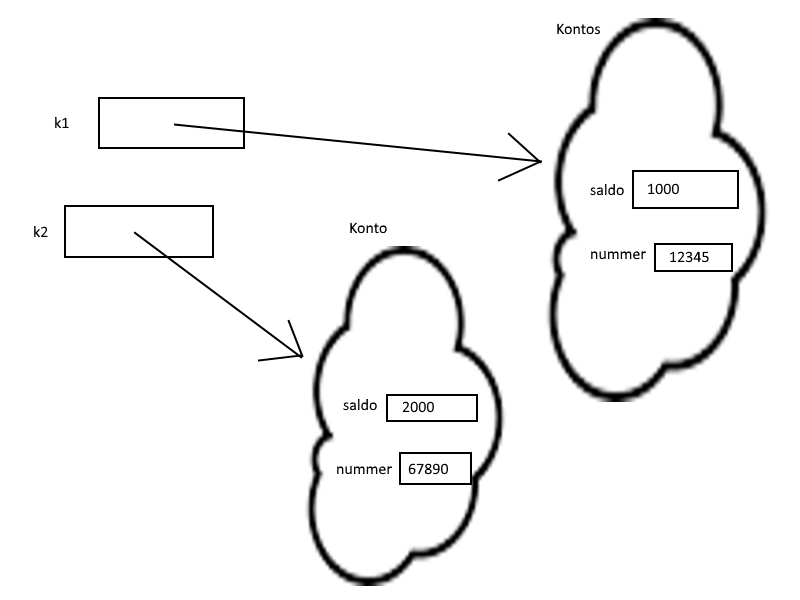
\includegraphics[scale=0.5]{../img/w04-solutions/uppgift-3a}
%
% \SubtaskSolved
% Tilldelningen på rad 8 \code{k1.nummer = 12345L} ger felmeddelande eftersom variablen är oföränderlig.
%
%
% \QUESTEND
%
%
%
%
% %%<AUTOEXTRACTED by mergesolu>%%      %Uppgift 3
%
%
%
%
% \WHAT{Klass med attribut som parametrar.}
%
% \QUESTBEGIN
%
% \Task  \what~  Om man vill ge attributen initialvärden när objektet skapas med \code{new}, kan man placera attributen i en parameterlista till klassen. Koden som körs när objektet skapas och attributen tilldelas sina initialvärden, kallas \textbf{konstruktor} \Eng{constructor}.
%
% \begin{REPL}
% scala> class Konto(var saldo: Int, val nummer: Long)
% scala> val k = new Konto(0, 12345L)
% scala> println("Konto: " + k.nummer + " Saldo:" + k.saldo)
% scala> println(k)
% scala> k.toString
% \end{REPL}
%
% \Subtask Den två sista raderna ovan skriver ut den identifierare som JVM använder för att hålla reda på objektet i sina interna datastrukturer. Vad skrivs ut?
%
% \Subtask Skapa ännu en instans av klassen Konto  med samma saldo och nummer som \code{k} ovan och spara den i \code{val k2} och undersök dess objektidentifierare. Får objekten \code{k} och \code{k2} olika objektidentifierare?
%
% \Subtask Sätt in olika belopp på respektive konto.
%
% \Subtask Vad händer om du försöker ändra attributet \code{nummer}?
%
% \Subtask\Pen Ibland räcker det fint med en tupel, men ofta vill man ha en klass istället. Beskriv några fördelar med en Konto-klassen ovan jämfört med en tupel av typen \code{(Int, Long)}.
%
% \begin{REPLnonum}
% scala> var k3 = (0, 12345L)
% scala> k3 = (k3._1 + 100, k3._2)
% \end{REPLnonum}
%
% \SOLUTION
%
%
% \TaskSolved \what
%
%
% \SubtaskSolved   \code{String = Konto@cd576}, där \code{Konto@cd576} är ett unikt namn som identifierar instansen.
%
% \SubtaskSolved   Ja.
%
% \SubtaskSolved
% \begin{REPLnonum}
% scala> k.saldo = 42
% scala> k2.saldo = 67
% \end{REPLnonum}
%
% \SubtaskSolved   Eftersom variablen är oföränderlig ges ett felmeddelande.
%
% \SubtaskSolved   En fördel med klass är att man kan specificera att variablen ska kunna vara föränderlig. En till är att man kan inkludera metoder i klassen som man vill kunna använda på värdena.
%
%
% \QUESTEND
%
%
%
%
% %%<AUTOEXTRACTED by mergesolu>%%      %Uppgift 4
%
%
%
%
% \WHAT{Publikt eller privat attribut?}
%
% \QUESTBEGIN
%
% \Task  \what~  Man kan förhindra att ett attribut syns utanför klassen med hjälp av nyckelordet \code{private}.
%
% \begin{REPL}
% scala> class Konto1(val nummer: Long){ var saldo = 0 }
% scala> val k1 = new Konto1(12345678901L)
% scala> k1.nummer
% scala> k1.saldo += 1000
% scala> class Konto2(val nummer: Long){ private var saldo = 0 }
% scala> val k2 = new Konto2(12345678901L)
% scala> k2.nummer
% scala> k2.saldo += 1000
% \end{REPL}
%
% \Subtask Vad händer ovan?
%
% \Subtask Gör en ny version av klassen \code{Konto} enligt nedan:
%
% \begin{Code}
% class Konto(val nummer: Long){
%   private var saldo = 0
%   def in(belopp: Int): Unit = {saldo += belopp}
%   def ut(belopp: Int): Unit = {saldo -= belopp}
%   def show: Unit =
%     println("Konto Nr: " + nummer + " saldo: " + saldo)
% }
%
% object Main {
%   def main(args: Array[String]): Unit = {
%     val k = new Konto(1234L)
%     k.show
%     k.in(1000)
%     println("Uttag: " + k.ut(500))
%     println("Uttag: " + k.ut(1000))
%     k.show
%   }
% }
% \end{Code}
%
% \Subtask Spara koden i en fil, kompilera med \code{scalac} och kör. Testa även vad som händer om du försöker komma åt attributet \code{saldo} i main-metoden med t.ex. \code{println(k.saldo)} eller \code{k.saldo += 1000}.
%
% \Subtask Vi ska nu förhindra överuttag. Ändra i metoden \code{ut} så att den får signaturen \code{ut(belopp: Int): (Int, Int) = ???} och implementera \code{ut} så att den returnerar både beloppet man verkligen kan ta ut och kvarvarande saldo. Om man försöker ta ut mer än det finns på kontot så ska saldot bli 0 och man får bara ut det som finns kvar. Spara, kompilera, kör.
%
% \Subtask Förbättra metoderna \code{in} och \code{ut} så att man inte kan sätta in eller ta ut negativa belopp.
%
% \Subtask Vad är fördelen med att göra föränderliga attribut privata och bara påverka deras värden indirekt via metoder?
%
% \SOLUTION
%
%
% \TaskSolved \what
%
%
% \SubtaskSolved
% Det går bra att ändra på variablen saldo i instansen av Konto1 men inte av Konto2 där man får ett error på raden ''k2.saldo += 1000''
%
% \SubtaskSolved  -
%
% \SubtaskSolved
% ''println(k.saldo)'' och ''k.saldo += 1000'' ger båda error, pga privat attribut.
%
% \SubtaskSolved
% \begin{Code}
% def ut(belopp: Int): (Int, Int) = {
% 	if(saldo >= belopp) {
% 		saldo -= belopp
% 		(belopp, saldo)
% 	} else {
% 		val temp = saldo
% 		saldo = 0
% 		(temp, 0)
% 	}
% }
% \end{Code}
%
% \SubtaskSolved
% Lägg till en if-sats i båda funktionerna som omsluter den gamla koden.
% \begin{Code}
% def ut(belopp: Int): (Int, Int) = {
%   if(belopp >= 0) {
%     if(saldo >= belopp) {
%       saldo -= belopp
%       (belopp, saldo)
%     } else {
%       val temp = saldo
%       saldo = 0
%       (temp, 0)
%     }
%   }
% }
%
% def in(belopp: Int): Unit = {
%   if(belopp >= 0) {
%     saldo += belopp
%   }
% }
% \end{Code}
%
% \SubtaskSolved
% Genom att göra attributet privat och gör egna metoder kan man se till att attriuten endast ändras på säkra sätt. Så inte fel uppstår.
%
%
% \QUESTEND
%
%
%
%
% %%<AUTOEXTRACTED by mergesolu>%%      %Uppgift 5
%
%
%
%
% \WHAT{Vilken typ har ett objekt?}
%
% \QUESTBEGIN
%
% \Task  \what~  Objektets typ bestäms av klassen. Vid tilldelning måste typerna passa ihop.
%
% \Subtask Vilka rader nedan ger felmeddelande? Hur lyder felmeddelandet?
% \begin{REPL}
% scala> class Punkt(val x: Double, val y: Double)
% scala> val pt: Punkt = new Punkt(10.0, 10.0)
% scala> val i: Int = pt.x
% scala> val (x: Double, y: Double) = (pt.x, pt.y)
% scala> val p: Double = new Punkt(5.0, 5.0)
% scala> val p = new Punkt(5.0, 5.0): Double
% scala> val p = new Punkt(5.0, 5.0): Punkt
% scala> pt: Punkt
% \end{REPL}
%
%
% \Subtask Man kan undersöka om ett objekt är av en viss typ med metoden \\ \code{isInstanceOf[Typnamn]}. Vad ger nedan anrop av metoden \code{isInstanceOf} för värde?
% \begin{REPL}
% scala> class Punkt(val x: Double, val y: Double)
% scala> val pt: Punkt = new Punkt(1.0, 2.0)
% scala> pt.isInstanceOf[Punkt]
% scala> pt.isInstanceOf[Double]
% scala> pt.x.isInstanceOf[Punkt]
% scala> pt.x.isInstanceOf[Double]
% scala> pt.x.isInstanceOf[Int]
% \end{REPL}
%
% \SOLUTION
%
%
% \TaskSolved \what
%
%
% \SubtaskSolved
% ''val i: Int = pt.x'' error: type mismatch;
% Eftersom typen Int ej är kompatibel med ett värde av typen Double.
%
% ''val p: Double = new Punkt(5.0, 5.0)'' error: type mismatch;
% Eftersom typen Double ej är kompatibel med ett värde av typen Punkt.
%
% ''val p = new Punkt(5.0, 5.0): Double'' error: type mismatch;
% Eftersom typen Double ej är kompatibel med ett värde av typen Punkt.
%
% \SubtaskSolved
% Rad 3 till 7 i respektive ordning: true, false, false, true och false.
%
%
% \QUESTEND
%
%
%
%
% %%<AUTOEXTRACTED by mergesolu>%%      %Uppgift 6
%
%
%
%
% \WHAT{Topptypen \code{Any}.}
%
% \QUESTBEGIN
%
% \Task  \what~ Alla klasser är också av typen \code{Any}. Alla klasser får därmed med sig några gemensamma metoder som finns i den fördefinierade klassen \code{Any}, däribland metoderna  \code{isInstanceOf} och \code{toString}.  Vad blir resultatet av respektive rad nedan? Vilken rad ger ett felmeddelande?
%
%
% \begin{REPL}
% scala> class Punkt(val x: Double, val y: Double)
% scala> val pt: Punkt = new Punkt(1.0, 2.0)
% scala> pt.isInstanceOf[Punkt]
% scala> pt.isInstanceOf[Any]
% scala> pt.x.toString
% scala> println(pt.x)
% scala> val a: Any = pt
% scala> println(a.x)
% scala> a.toString
% scala> pt.y.toString
% scala> a.y.toString
% \end{REPL}
%
% \SOLUTION
%
%
% \TaskSolved \what
%
% \begin{enumerate}
% \item Definierar klassen Punkt.
% \item En variabel pt: Punkt skapas.
% \item true
% \item true
% \item String = 1.0
% \item skriver ut: 1.0
% \item En variabel med namnet a skapas med typen Any.
% \item error: value x is not a member of Any
% \item a ges nu typen String
% \item String = 2.0
% \item error: value y is not a member of Any
% \end{enumerate}
%
%
% \QUESTEND
%
%
%
%
% %%<AUTOEXTRACTED by mergesolu>%%      %Uppgift 7
%
%
%
%
% \WHAT{Byta ut metoden \code{toString}}.
%
% \QUESTBEGIN
%
% \Task  \what~ I klassen \code{Any} finns metoden \code{toString} som skapar en strängrepresentation av objektet. Du kan byta ut metoden \code{toString} i klassen \code{Any} mot din egen implementation. Man använder nyckelordet \code{override} när man vill byta ut en metodimplementation.
%
% \begin{REPL}
% scala> class Punkt(val x: Double, val y: Double) {
%          override def toString: String = "[x=" + x + ",y=" + y + "]"
%        }
% scala> val pt = new Punkt(1.0, 42.0)
% scala> pt.toString
% scala> println(pt)
% \end{REPL}
%
% \Subtask Vad händer egentligen på sista raden ovan?
%
% \Subtask Omdefiniera toString så att den ger en sträng på formen \code{Punkt(1.0, 42.0)}.
%
% \Subtask Vad händer om du utelämnar nyckelordet \code{override} vid omdefiniering?
%
% \SOLUTION
%
%
% \TaskSolved \what
%
%
% \SubtaskSolved
% ''println(pt)'' kallar på pt.toString, och eftersom metoden är överskriven kallas den nya version.
%
% \SubtaskSolved   \code{override def toString: String = ''Punkt('' + x + '', '' + y + '').''}
%
% \SubtaskSolved
% error: overriding method toString in class Object of type ()String;
%
%
% \QUESTEND
%
%
%
%
% %%<AUTOEXTRACTED by mergesolu>%%      %Uppgift 8
%
%
%
%
% \WHAT{Objektfabrik med \code{apply}-metod.}
%
% \QUESTBEGIN
%
% \Task  \what~  Man kan ordna så att man slipper skriva \code{new} med ett s.k. \emph{fabriksobjekt} \Eng{factory object}.
% \begin{Code}
% class Pt(val x: Double, y: Double) {
%   override def toString: String = "Pt(x=" + x + ",y=" + y + ")"
% }
% object Pt {
%   def apply(x: Double, y: Double): Pt = new Pt(x, y)
% }
% \end{Code}
%
% \Subtask Skriv satser som använder metoden \code{apply} i fabriksobjektet \code{object Pt} för att skapa flera olika punkter.
%
% \Subtask Ge applymetoden default-argument 0.0 för både x och y så att \code{Pt()} skapar en punkt i origo.
%
% \Subtask Skapa en klass \code{Rational} som representerar rationellt tal som en kvot mellan två heltal. Ge klassen två oföränderliga, publika klassparameterattribut med namnen \code{nom} för täljaren och \code{denom} för nämnaren.
%
% \Subtask Skapa ett fabriksobjekt med en \code{apply}-metod som tar två heltalsparametrar och skapar en instans av klassen \code{Rational}.
%
% \Subtask Skapa olika instanser av din klass \code{Rational} ovan med hjälp av fabriksobjektet.
%
%
% \SOLUTION
%
%
% \TaskSolved \what
%
%
% \SubtaskSolved
% \begin{REPL}
% scala> val pt = Pt(1.0, 2.0)
% pt: Pt = Pt(x=1.0,y=2.0)
%
% scala> Pt(4.0, 2.0)
% res0: Pt = Pt(x=4.0,y=2.0)
%
% scala> Pt(6.0, 3.0)
% res1: Pt = Pt(x=6.0,y=3.0)
%
% scala> Pt(666.0, 1337.0)
% res2: Pt = Pt(x=666.0,y=1337.0)
% \end{REPL}
%
% \SubtaskSolved  \code{def apply(): Pt = new Pt(0, 0)}
%
% \SubtaskSolved  \code{class Rational(val nom: Int, val denom: Int)}
%
% \SubtaskSolved
% \begin{REPLnonum}
% object Rational {
% def apply(nom: Int, denom: Int): Rational = new Rational(nom, denom)
% }
% \end{REPLnonum}
%
% \SubtaskSolved
% \begin{REPL}
% scala> Rational(2, 5)
% scala> Rational(2, 7)
% scala> Rational(7, 4)
% scala> Rational(666, 1337)
% \end{REPL}
%
%
% \QUESTEND
%
%
%
%
% %%<AUTOEXTRACTED by mergesolu>%%      %Uppgift 9
%
%
%
%
% \WHAT{Skapa en case-klass.}
%
% \QUESTBEGIN
%
% \Task  \what~  Med en case-klass får man \code{toString} och fabriksobjekt på köpet. Man behöver inte skriva \code{val} framför klassparametrar i case-klasser; klassparametrar blir publika, oföränderliga attribut automatiskt när man deklarerar en case-klass.
%
% \begin{REPL}
% scala> case class Pt(x: Double, y: Double)
% scala> val p = Pt(1.0, 42.0)
% scala> p.toString
% scala> println(p)
% scala> println(Pt(5,6))
% \end{REPL}
%
% \Subtask Implementera din klass \code{Rational} från föregående uppgift, men nu som en case-klass.
%
% \SOLUTION
%
%
% \TaskSolved \what
%
% \SubtaskSolved  \code{case class Rational(nom: Int, denom: Int)}
%
%
% \QUESTEND
%
%
%
%
% %%<AUTOEXTRACTED by mergesolu>%%      %Uppgift 10
%
%
%
%
% \WHAT{Metoder på datastrukturer.}
%
% \QUESTBEGIN
%
% \Task \label{task:point} \what~   En datastruktur blir mer användbar om det finns metoder som kan användas på datastrukturen. Metoder i Scala kan även ha (vissa) specialtecken som namn, t.ex. \code{+} enligt nedan.
% \begin{REPL}
% scala> case class Point(x: Double, y: Double) {
%          def distToOrigin: Double = math.hypot(x, y)
%          def add(p: Point): Point = Point(x + p.x, y + p.y)
%          def +(p: Point): Point = add(p)
%        }
% \end{REPL}
%
% \Subtask Använd metoden \code{distToOrigin} för att ta reda på vad punkten med koordinaterna (3, 4) har för avstånd till origo?
%
% \Subtask Skriv satser som skapar två punkter (3,4) och (5, 6) och låt variablerna p1 och p2 referera till respektive punkt. Låt variabeln p3 bli summan av p1 och p2 med hjälp av metoden \code{add}. Vad får uttrycken \code{p3.x} resp. \code{p3.y} för värden?
%
%
%
% \SOLUTION
%
%
% \TaskSolved \what
%
%
% \SubtaskSolved
% \begin{REPLnonum}
% scala> Point(3, 4).distToOrigin
% res0: Double = 5.0
% \end{REPLnonum}
%
% \SubtaskSolved
% p3.x = 8
% p3.y = 10
%
%
% \QUESTEND
%
%
%
%
% %%<AUTOEXTRACTED by mergesolu>%%      %Uppgift 11
%
%
%
%
% \WHAT{Operatornotation.}
%
% \QUESTBEGIN
%
% \Task  \what~  Vid punktnotation på formen: \\ \code{objekt.metod(argument)} \\ kan man skippa punkten och parenteserna och skriva:\\ \code{objekt metod argument}  \\
% Detta förenklade skrivsätt kallas \textbf{operatornotation}.
%
% \Subtask Använd klassen \code{Point} från uppgift \ref{task:point} och prova nedan satser. Vilka rader använder operatortnotation och vilka rader använder punktnotation? Vilka rader ger felmeddelande?
% \begin{REPL}
% scala> val p1 = Point(3,4)
% scala> val p2 = Point(3,4)
% scala> p1.add(p2)
% scala> p1 add p2
% scala> p1.+(p2)
% scala> p1 + p2
% scala> 42 + 1
% scala> 42.+(1)
% scala> 42.+ 1
% scala> 42 +(1)
% scala> 1.to(42)
% scala> 1 to 42
% scala> 1.to(42)
% \end{REPL}
%
% \Subtask Implementera metoderna \code{sub} och \code{-} i klassen \code{Point} och skriv uttryck som kombinerar add och sub, samt + och - i både punktnotation och operatornotation.
%
% \Subtask Operatornotation fungerar även med flera argument. Man använder då parenteser om listan med argumenten:
% \code{ objekt metod (arg1, arg2)}  \\
% Definiera en metod \\
% \code{def scale(a: Double, b: Double) = Point(x * a, y * b)} \\
% i klassen \code{Point} och skriv satser som använder metoden med punktnotation och operatornotation.
%
%
%
%
%
% \SOLUTION
%
%
% \TaskSolved \what
%
%
% \SubtaskSolved
% \\Operatornotation:	4, 6, 10, 12
% \\Punktnotation:		3, 5, 8, 9, 11, 13
% \\Felmeddelande:		9
%
% \SubtaskSolved
% \begin{Code}
% case class Point(x: Double, y: Double) {
%   def distToOrigin: Double = math.hypot(x, y)
%   def add(p: Point): Point = Point(x + p.x, y + p.y)
%   def +(p: Point): Point = add(p)
%   def sub(p: Point): Point = Point(x - p.x, y - p.y)
%   def -(p: Point): Point = sub(p)
% }
% \end{Code}
% \begin{REPL}
% scala> val p1: Point = Point(1, 9)
% scala> val p2: Point = Point(9, 6)
% scala> p1.sub(p2)
% scala> p1.-(p2)
% scala> p2 sub p1
% scala> p2 - p2
% scala> p1.add(p2.sub(p1))
% scala> p1 + (p2 - p1)
% \end{REPL}
%
% \SubtaskSolved
% \begin{Code}
% case class Point(x: Double, y: Double) {
%   def distToOrigin: Double = math.hypot(x, y)
%   def add(p: Point): Point = Point(x + p.x, y + p.y)
%   def +(p: Point): Point = add(p)
%   def sub(p: Point): Point = Point(x - p.x, y - p.y)
%   def -(p: Point): Point = sub(p)
%   def scale(a: Double, b: Double) = Point(x * a, y * b)
% }
% \end{Code}
% \begin{REPL}
% scala> val p: Point(13,  37)
% scala> p.scale(4, 2)
% scala> p scale (3, 7)
% \end{REPL}
%
%
% \QUESTEND
%
%
%
%
% %%<AUTOEXTRACTED by mergesolu>%%      %Uppgift 12
%
%
%
%
% \WHAT{Föränderlighet och oföränderlighet.}
%
% \QUESTBEGIN
%
% \Task  \what~  Oföränderliga och föränderliga objekt beter sig olika vid tilldelning.
%
% \Subtask\Pen Innan du kör nedan kod: Försök lista ut vad som kommer att skrivas ut. Rita minnessituationen efter varje tilldelning.
%
% \begin{Code}
% println("\n--- Example 1: mutable value assigmnent")
% var x1 = 42
% var y1 = x1
% x1 = x1 + 42
% println(x1)
% println(y1)
% \end{Code}
%
% \Subtask\Pen Innan du kör nedan kod: Försök lista ut vad som kommer att skrivas ut. Rita minnessituationen efter varje tilldelning.
%
% \begin{Code}
% println("\n--- Example 2: mutable object reference assignment")
% class MutableInt(private var i: Int) {
%   def +(a: Int): MutableInt = { i = i + a; this }
%   override def toString: String = i.toString
% }
% var x2 = new MutableInt(42)
% var y2 = x2
% x2 = x2 + 42
% println(x2)
% println(y2)
% \end{Code}
%
% \Subtask\Pen Innan du kör nedan kod: Försök lista ut vad som kommer att skrivas ut. Rita minnessituationen efter varje tilldelning.
%
% \begin{Code}
% println("\n--- Example 3: immutable object reference assignment")
% class ImmutableInt(val i: Int) {
%   def +(a: Int): ImmutableInt = new ImmutableInt(i + a)
%   override def toString: String = i.toString
% }
% var x3 = new ImmutableInt(42)
% var y3 = x3
% x3 = x3 + 42
% println(x3)
% println(y3)
% \end{Code}
%
% \Subtask\Pen Vad finns det för fördelar med oföränderliga datastrukturer?
%
%
% \SOLUTION
%
%
% \TaskSolved \what
%
%
% \SubtaskSolved   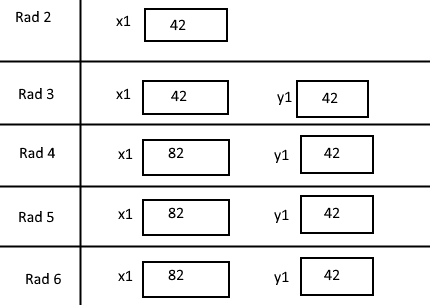
\includegraphics[scale=0.5]{../img/w04-solutions/uppgift-13a}
%
% \SubtaskSolved
% \begin{enumerate}
% \item 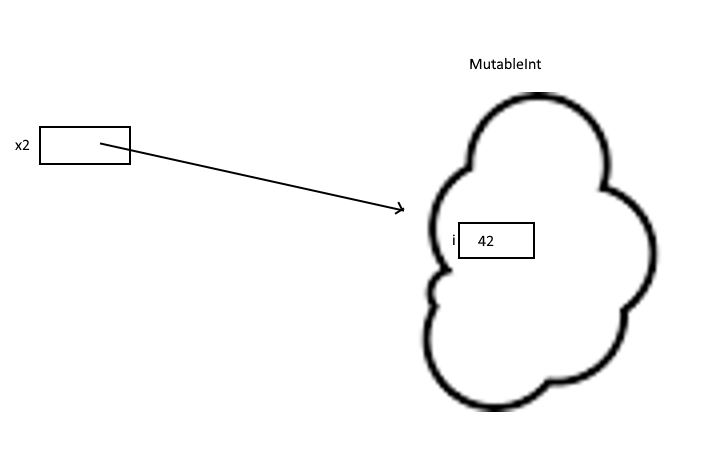
\includegraphics[scale=0.5]{../img/w04-solutions/uppgift-13b-1}
% \item 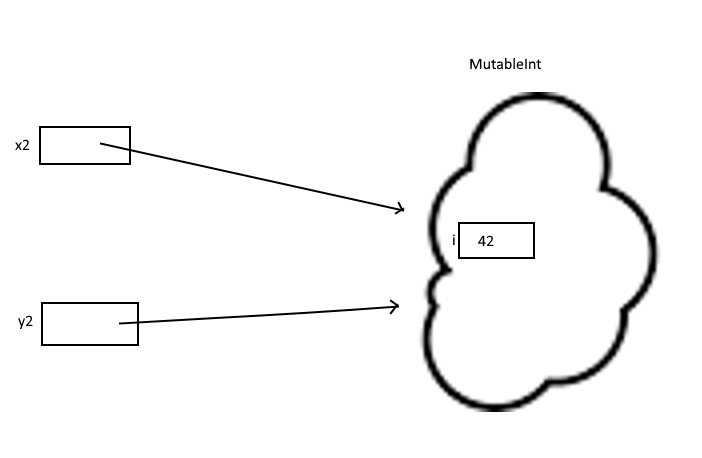
\includegraphics[scale=0.5]{../img/w04-solutions/uppgift-13b-2}
% \item 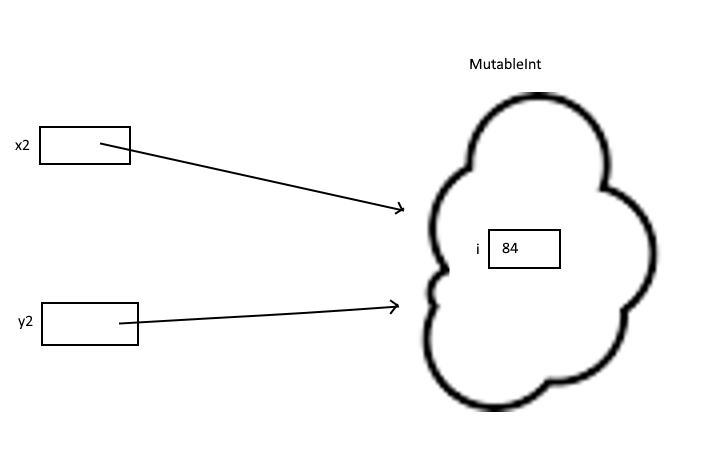
\includegraphics[scale=0.5]{../img/w04-solutions/uppgift-13b-3}
% \end{enumerate}
%
% \SubtaskSolved
% \begin{enumerate}
% \item 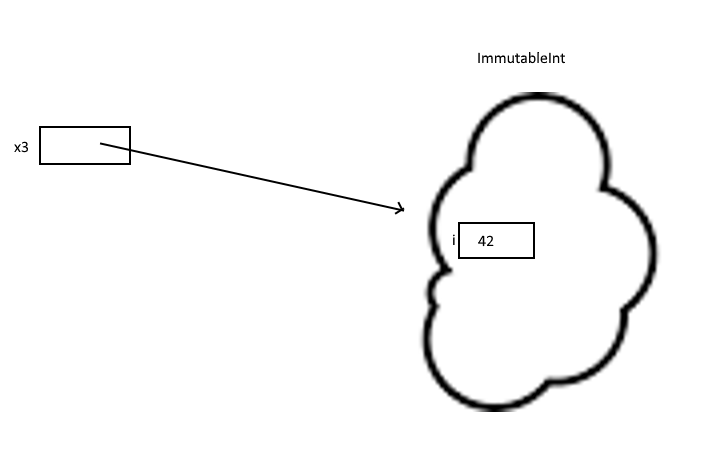
\includegraphics[scale=0.5]{../img/w04-solutions/uppgift-13c-1}
% \item 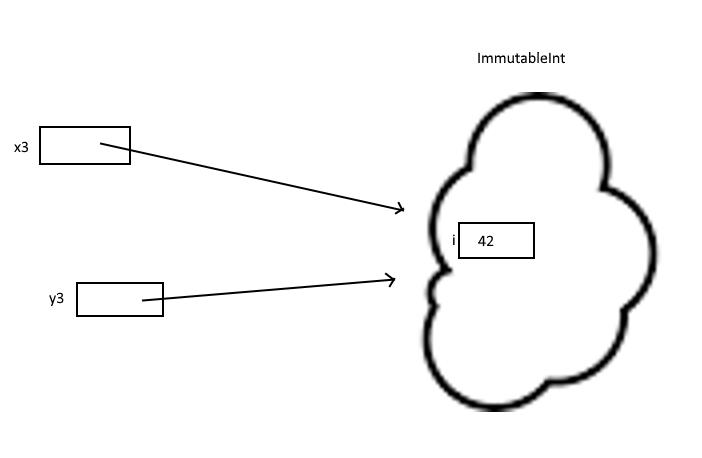
\includegraphics[scale=0.5]{../img/w04-solutions/uppgift-13c-2}
% \item 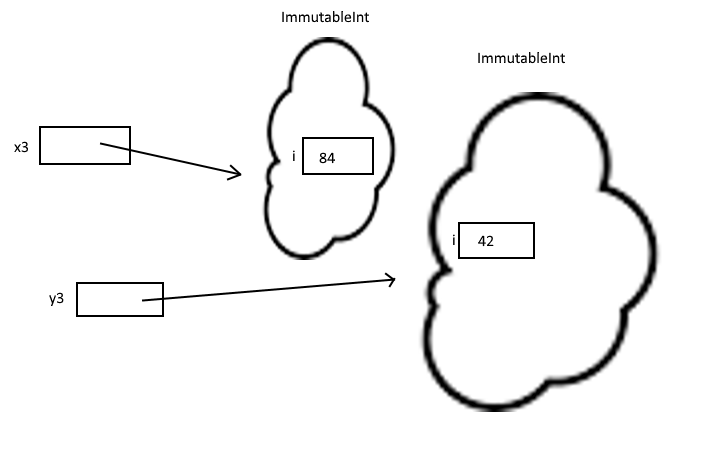
\includegraphics[scale=0.5]{../img/w04-solutions/uppgift-13c-3}
% \end{enumerate}
%
% \SubtaskSolved   En stor fördel är att vi till exempel kan skicka med en immutable som argument till en metod och vara säkra på att metoden inte ändrar på värdet.
%
%
% \QUESTEND
%
%
%
%
% %%<AUTOEXTRACTED by mergesolu>%%      %Uppgift 13
%
%
%
%
% \WHAT{Några användbara samlingar.}
%
% \QUESTBEGIN
%
% \Task  \what~  En \textbf{samling} \Eng{collection} är en datastruktur som samlar många objekt av samma typ. I \code{scala.collection} och \code{java.util} finns många olika samlingar med en uppsjö användbara metoder. De olika samlingarna i \code{scala.collection} är ordnade i en gemensam hierarki med många gemensamma metoder; därför har man nytta av det man lär sig om metoderna i en Scala-samling när man använder en annan samling. Vi har redan tidigare sett samlingen \code{Vector}:
%
% \begin{REPL}
% scala> val tärningskast = Vector.fill(10000)((math.random * 6 + 1).toInt)
% scala> tä   // tryck TAB
% scala> tärningskast.  // tryck TAB
% \end{REPL}
%
% \Subtask Ungefär hur många metoder finns det som man kan göra på objekt av typen \code{Vector}? Det är svårt att lära sig alla dessa på en gång, så vi väljer ut några få i kommande uppgifter.
%
% \Subtask Jämför överlappet mellan metoderna i \code{Vector} och \code{List} och uppskatta hur stor andel av metoderna som är gemensamma:
% \begin{REPL}
% scala> val myntkast =
%          List.fill(10000)(if (math.random < 0.5) "krona" else "klave")
% scala> my   // tryck TAB
% scala> myntkast.  // tryck TAB
% \end{REPL}
%
% \SOLUTION
%
%
% \TaskSolved \what
%
%
% \SubtaskSolved   Ungefär 150 metoder.
%
% \SubtaskSolved   Ungefär lika många.
%
%
% \QUESTEND
%
%
%
%
% %%<AUTOEXTRACTED by mergesolu>%%      %Uppgift 14
%
%
%
%
% \WHAT{Typparameter.}
%
% \QUESTBEGIN
%
% \Task  \what~  Vissa funktioner är generella för många typer och tar en så kallad \textbf{typparameter} inom hakparenteser. Ofta slipper man skriva typparametrar, då kompilatorn kan härleda typen utifrån argumenten. Om man anger typparametrar explicit så hjälper kompilatorn dig med att kolla att det verkligen är rätt typ i samlingen.
%
% \Subtask Vad händer nedan?
% \begin{REPL}
% scala> var xs = Vector.empty[Int]
% scala> xs = xs :+ "42"
% scala> xs = xs :+ 43 :+ 64 :+ 46
% scala> xs
% scala> xs :+= "42".toInt
% scala> var ys = Vector[Int]("ett", "två", "tre")
% scala> var ingenting = Vector.empty
% scala> ingenting = Vector(1,2,3)
% \end{REPL}
%
% \Subtask Samlingar är mer användbara om de är \emph{generiska}, vilket innebär att elementens typ avgörs av en typparameter och därför kan vara av vilken typ som helst. Man kan definiera egna funktioner som tar generiska samlingar som parametrar. Förklara vad som händer här:
% \begin{REPL}
% scala> val vego = Vector("gurka", "tomat", "apelsin", "banan")
% scala> val prim = Vector(2, 3, 5, 7, 11, 13)
% scala> def först[T](xs: Vector[T]): T = xs.head
% scala> def sist[T](xs: Vector[T]) = xs.last
% scala> def förstOchSist[T](xs: Vector[T]): (T, T) = (xs.head, xs.last)
% scala> först(vego)
% scala> sist(prim)
% scala> förstOchSist(vego)
% scala> förstOchSist(prim)
% scala> def wrap[T](pair: (T, T))(xs: Vector[T]) = pair._1 +: xs :+ pair._2
% scala> wrap("Odla", "och ät!")(vego)
% scala> wrap("Odla", "och ät!")(vego).mkString(" ")
% \end{REPL}
%
%
%
%
%
% \SOLUTION
%
%
% \TaskSolved \what
%
%
% \SubtaskSolved
% \\1. Instansierar en tom vektor med element av typen int och tilldelar värdet till en variabel xs.
% \\2. Error eftersom \code{xs :+ ''42''} ger en Vector[Any] när Vector[Int] krävs.
% \\3. xs tilldelas ett nytt värde av Vector(43, 64, 46)
% \\4. xs skrivs ut.
% \\5. Lägger till talet 42 i xs.
% \\6. Error: type mismatch
% \\7. Skapar en tom Vector i variablen ingenting
% \\8. error: type mismatch; found: Int(3), required: Nothing
%
% \SubtaskSolved
% Tre metoder skapas: den första för att få första elementet i en lista, och eftersom den definieras med specialtypen T går den att använda med alla vektorer oavsett typen av variabeln i vektorn. Den andra får fram sista elementet och den sista hämtar båda två.
%
% En till function definieras längre ner med  namnet ''wrap'', som tar en lista och lägger till ett element längst fram och ett längst bak.
%
%
% \QUESTEND
%
%
%
%
% %%<AUTOEXTRACTED by mergesolu>%%      %Uppgift 15
%
%
%
%
% \WHAT{Några viktiga samlingsmetoder.}
%
% \QUESTBEGIN
%
% \Task  \what~  Deklarera följande vektorer i REPL.
% \begin{REPL}
% scala> val xs = (1 to 10).toVector
% scala> val a = Vector("abra", "ka", "dabra")
% scala> val b = Vector( "sim", "sala", "bim", "sala", "bim")
% scala> val stor = Vector.fill(100000)(math.random)
% \end{REPL}
% Undersök i REPL vad som händer nedan. Alla dessa metoder fungerar på alla samlingar som är indexerbara sekvenser. Givet deklarationerna ovan: vad har uttrycken nedan för värde och typ? Förklara vad som händer hälp av denna  översikt: \href{http://docs.scala-lang.org/overviews/collections/seqs}{docs.scala-lang.org/overviews/collections/seqs}
%
% \Subtask \code{a(1) + xs(1)}
%
% \Subtask \code{a apply 0}
%
% \Subtask \code{a.isDefinedAt(3)}
%
% \Subtask \code{a.isDefinedAt(100)}
%
% \Subtask \code{stor.length}
%
% \Subtask \code{stor.size}
%
% \Subtask \code{stor.min}
%
% \Subtask \code{stor.max}
%
% \Subtask \code{a indexOf "ka"}
%
% \Subtask \code{b.lastIndexOf("sala")}
%
% \Subtask \code{"först" +: b   //minnesregel: colon on the collection side}
%
% \Subtask \code{a :+ "sist"    //minnesregel: colon on the collection side}
%
% \Subtask \code{xs.updated(2,42)}
%
% \Subtask \code{a.padTo(10, "!")}
%
% \Subtask \code{b.sorted}
%
% \Subtask \code{b.reverse}
%
% \Subtask \code{a.startsWith(Vector("abra", "ka"))}
%
% \Subtask \code{"hejsan".endsWith("san")}
%
% \Subtask \code{b.distinct}
%
%
%
% \SOLUTION
%
%
% \TaskSolved \what
%
%
% \SubtaskSolved   String = ''ka2''
%
% \SubtaskSolved   String = ''abra''
%
% \SubtaskSolved   false
%
% \SubtaskSolved   false
%
% \SubtaskSolved   100000
%
% \SubtaskSolved   100000
%
% \SubtaskSolved   minsta talet i listan
%
% \SubtaskSolved   största talet i listan
%
% \SubtaskSolved   1
%
% \SubtaskSolved   3
%
% \SubtaskSolved   Vektor b fast med ''först'' som första element
%
% \SubtaskSolved   Vektor a fast med ''sist'' som sista element.
%
% \SubtaskSolved   plats 3 i vektorn xs får värdet 42
%
% \SubtaskSolved   En ny vektor fylld med ''!'' från och med plats 4 till 10. Men de andra värdena samma som i a.
%
% \SubtaskSolved   b sorterad i bokstavsordning
%
% \SubtaskSolved   b baklänges
%
% \SubtaskSolved   true
%
% \SubtaskSolved   true
%
% \SubtaskSolved   en vektor med alla unika element i b.
%
%
% \QUESTEND
%
%
%
%
% %%<AUTOEXTRACTED by mergesolu>%%      %Uppgift 16
%
%
%
%
% \WHAT{Några generella samlingsmetoder.}
%
% \QUESTBEGIN
%
% \Task  \what~  Det finns metoder som går att köra på \emph{alla} samlingar även om de inte är indexerbara. Givet deklarationerna i föregående uppgift: vad har uttrycken nedan för värde och typ? Förklara vad som händer med hjälp av dessa översikter: \\ \href{http://docs.scala-lang.org/overviews/collections/trait-traversable}{docs.scala-lang.org/overviews/collections/trait-traversable} \\ \href{http://docs.scala-lang.org/overviews/collections/trait-iterable}{docs.scala-lang.org/overviews/collections/trait-iterable}
%
% \Subtask \code{a ++ b}
%
% \Subtask \code{a ++ stor}
%
% \Subtask \code{val ys = xs.map(_ * 5)}
%
% \Subtask \code{b.toSet     // En mängd har inga dubletter}
%
% \Subtask \code{a.head + b.last}
%
% \Subtask \code{a.tail}
%
% \Subtask \code{a.head +: a.tail == a}
%
% \Subtask \code{Vector(a.head) ++ Vector(b.last)}
%
% \Subtask \code{a.take(1) ++ b.takeRight(1)}
%
% \Subtask \code{a.drop(2) ++ b.drop(1).dropRight(2)}
%
% \Subtask \code{a.drop(100)}
%
% \Subtask \code{val e = Vector.empty[String]; e.take(100)}
%
% \Subtask \code{Vector(e.isEmpty, e.nonEmpty)}
%
% \Subtask \code{a.contains("ka")}
%
% \Subtask \code{"ka" contains "a"}
%
% \Subtask \code{a.filter(s => s.contains("k")) }
%
% \Subtask \code{a.filter(_.contains("k")) }
%
% \Subtask \code{a.map(_.toUpperCase).filterNot(_.contains("K")) }
%
% \Subtask \code{xs.filter(x => x % 2 == 0)}
%
% \Subtask \code{xs.filter(_ % 2 == 0)}
%
%
% \SOLUTION
%
%
% \TaskSolved \what
%
%
% \SubtaskSolved
% Metoden ger tillbaka en ny Vector[String] som nu består av alla element i a plus alla element i b. I samma ordning med elementen i a först.
%
% \SubtaskSolved
% Samma som i uppgift a fast vektorn som returnas är av typen Vector[Any]. Det är eftersom Any är den närmsta typen som String och Double delar. Elementen från vektor a är fortfarande först och uppföljt av elementen i stor.
%
% \SubtaskSolved
% Variablen ys får värdet av en Vector[Int] som innehåller alla talen från xs fast multiplicerade med 5. Alltså ys = 5, 10, 15..., osv.
%
% \SubtaskSolved
% Functionen tar alla värden från en Vektor och sätter in i ett Set (mängd). Eftersom en mängd ej har dubletter så försvinner ett ''sala'' och ett ''bim'', Vector[String] som returneras blir därför (''sim'', ''sala'', ''bim'').
%
% \SubtaskSolved
% Metoden head ger första elementet i en samling, och last sista. Därför blir kombinationen av a.head och b.last en ny Vector[String] som består av a:s första element, och b:s första element.
%
% \SubtaskSolved
% Ger en Vector[String] som innehåller alla element efter det första. Alltså i detta fallet ''ka'' och ''dabra''.
%
% \SubtaskSolved
% True, eftersom head ger första elementet och tail ger resten, sedan sätter metoden +: ihop dem till en vektor med samma värden som a.
%
% \SubtaskSolved
% Eftersom ++ sätter ihop alla värden från två vektorer måste vi först omvandla från en sträng till vektor. Resultatet blir en ny vektor av samma typ som innan med a:s första element och b:S sista.
%
% \SubtaskSolved
% Samma resultat som i h, metoden take börjar från vänster och tar så många element som man skickar med som parameter och gör till en ny lista. Med 1 som parameter motsvarar det att göra Vector(a.head). Metoden takeRight gör samma sak fast från höger.
%
% \SubtaskSolved
% Metoden drop är motsvarigheten till take fast exkluderar de specifierade elementen istället för att inkludera dem i vektorn.
%
% \SubtaskSolved
% Eftersom a endast innehåller 3 element returnerar drop(100) en tom vektor.
%
% \SubtaskSolved
% Returnerar en tom vektor med element typen String
%
% \SubtaskSolved
% returnerar Vector(true, false)
%
% \SubtaskSolved
% True, metoden contains kollar om en samling innehåller ett specifikt element.
%
% \SubtaskSolved
% True. Eftersom en sträng även kan ses som Vector[Char].
%
% \SubtaskSolved
% Filtrerar vektorn a till att endast innehålla strängar som innehåller k.
%
% \SubtaskSolved
% Exakt samma som i p
%
% \SubtaskSolved
% map(\_.toUpperCase) omvandlar alla strängar i a till stora bokstäver
% filterNot(\_.contains(''K'')) tar resultatet vi precis fick och tar bort alla strängar som innehåller stora K.
%
% \SubtaskSolved
% filtrerar så att endast jämna tal finns kvar.
%
% \SubtaskSolved
% Exakt samma som i s
%
%
%
%
% \QUESTEND
%
%
%
%
% %%<AUTOEXTRACTED by mergesolu>%%      %Uppgift 17
%
%
%
%
% \WHAT{NEEDS A TOPIC DESCRIPTION}
%
% \QUESTBEGIN
%
% \Task  \what~ De olika samlingarna i \code{scala.collection} används flitigt i andra paket, exempelvis \code{scala.util} och \code{scala.io}.
%
% \Subtask Vad händer här? (Metoden \code{shuffle} skapar en ny samling med elementen i slumpvis ordning.)
% \begin{REPL}
% val xs = Vector(1,2,3)
% def blandat = scala.util.Random.shuffle(xs)
% def test = if (xs == blandat) "lika" else "olika"
% (for(i <- 1 to 100) yield test).count(_ == "lika")
% \end{REPL}
%
%
% \Subtask Skapa en textfil med namnet \code{fil.txt} som innehåller lite text och läs in den med: \\\code{scala.io.Source.fromFile("fil.txt", "UTF-8").getLines.toVector}
% \begin{REPL}
% > cat > fil.txt
% hejsan
% svejsan
% > scala
% scala> val xs = scala.io.Source.fromFile("fil.txt", "UTF-8").getLines.toVector
% scala> xs.foreach(println)
% \end{REPL}
%
%
% \Subtask Vad händer här? (Metoden \code{trim} på värden av typen \code{String} ger en ny sträng med blanktecken i början och slutet borttagna.)
% \begin{REPL}
% scala> val pgk =
%   scala.io.Source.fromURL("http://cs.lth.se/pgk/","UTF-8").getLines.toVector
% scala> pgk.foreach(println)
% scala> pgk.map(_.trim).
%          filterNot(_.startsWith("<")).
%          filterNot(_.isEmpty).
%          foreach(println)
% \end{REPL}
%
%
%
% \SOLUTION
%
%
% \TaskSolved \what
%
%
% \SubtaskSolved
% Vi instansierar en vektor xs med talen 1, 2 och 3.
% sedan definierar vi en metod blandat som ger oss en randomiserad version av xs.
% sedan definierar vi en till metod som testar om xs är lika med resultatet från blandat. Om det är så returnerar den strängen ''lika'' annars ''olika''.
% Sist kör vi en for-loop där vi 100 gånger kör testet, samtidigt räknas hur många gånger ''lika'' returneras.
%
% Vårt resultat är en siffra på hur många gånger xs var samma som en blandad version av sig själv, eftersom det finns 6 permutationer med 3 variabler så borde det vara ungefär 1/6 chans.
%
% \SubtaskSolved  -
%
% \SubtaskSolved
% \\ \code{map(\_.trim)} tar bort alla onödiga mellanrum i början och slutet på varje rad
% \\ \code{filterNot(\_.startsWith(''<''))} filtrerar bort alla rader som börjar med strängen ''<''
% \\ \code{filterNot(\_.isEmpty)} filtrerar bort alla tomma rader.
% \\ \code{foreach(println)} skriver ut alla rader.
%
%
% \QUESTEND
%
%
%
%
% %%<AUTOEXTRACTED by mergesolu>%%      %Uppgift 18
%
%
%
%
% \WHAT{Jämföra List och Vector.}
%
% \QUESTBEGIN
%
% \Task  \what~  En indexerbar sekvens av värden kallas vektor eller lista. I Scala finns flera klasser som kan kan indexeras, däribland klasserna \code{Vector} och \code{List}.
%
% \Subtask \emph{Likheter mellan \code{Vector} och \code{List}.} Kör nedan rader i REPL. Prova indexera i båda och studera hur stor andel av metoderna som är gemensamma.
% \begin{REPL}
% scala> val sv = Vector("en", "två", "tre", "fyra")
% scala> val en = List("one", "two", "three", "four")
% scala> sv(0) + sv(3)
% scala> en(0) + en(3)
% scala> sv. //tryck TAB
% scala> en. //tryck TAB
% \end{REPL}
%
% \Subtask \emph{Skillnader mellan \code{Vector} och \code{List}.} Klassen \code{Vector} i Scala har ''under huven'' en avancerad datastruktur i form av ett s.k. självbalanserande träd, vilket gör att \code{Vector} är snabbare än \code{List} på nästan allt, \emph{utom} att bearbeta elementen i \emph{början} av sekvensen; vill man lägga till och ta bort i början av en \code{List} så kan det ibland gå ungefär dubbelt så fort jämfört med \code{Vector}, medan alla andra operationer är lika snabba eller snabbare med \code{Vector}. Det finns ett fåtal speciella metoder, som bara finns i \code{List}, för att skapa en lista och lägga till i början av en lista. Vad händer nedan?
%
% \begin{REPL}
% scala> var xs = "one" :: "two" :: "three" :: "four" :: Nil
% scala> xs = "zero" :: xs
% scala> val ys = xs.reverse ::: xs
% \end{REPL}
%
%
% \SOLUTION
%
%
% \TaskSolved \what
%
%
% \SubtaskSolved
% I princip alla metoder delas, en lista har några fler t. ex. ''::'', '':::'', ''mapConserve'' osv.
%
% \SubtaskSolved
% Först skapas en lista med 4 sträng värden och instansierar variablen xs med det värdet.
% sedan skapar vi en ny lista, som består av ''zero'' + den gamla listan och ger värdet till xs.
% Sist instansierar vi en ny variabel ys, som får värdet av xs omvänd plus xs.
%
%
% \QUESTEND
%
%
%
%
% %%<AUTOEXTRACTED by mergesolu>%%      %Uppgift 19
%
%
%
%
% \WHAT{Mängd.}
%
% \QUESTBEGIN
%
% \Task  \what~  En mängd är en samling som garanterar att det inte finns några dubbletter. Det går dessutom väldigt snabbt, även i stora mängder, att kolla om ett element finns eller inte i mängden. Elementen i samlingen \code{Set} hamnar ibland, av effektivitetsskäl, i en förvånande ordning.
% \begin{REPL}
% scala> val s = Set("Malmö", "Stockholm", "Göteborg", "Köpenhamn", "Oslo")
% s: scala.collection.immutable.Set[String] =
%      Set(Oslo, Malmö, Köpenhamn, Stockholm, Göteborg)
%
% scala> val t = Set("Sverige", "Sverige", "Sverige", "Danmark", "Norge")
% t: scala.collection.immutable.Set[String] = Set(Sverige, Danmark, Norge)
% \end{REPL}
% Givet ovan deklarationer: vad blir värde och typ av nedan uttryck?
%
% \Subtask \code{s + "Malmö" == s}
%
% \Subtask \code{s ++ t}
%
% \Subtask \code{Set("Malmö", "Oslo").subsetOf(s)}
%
% \Subtask \code{s subsetOf Set("Malmö", "Oslo")}
%
% \Subtask \code{s contains "Lund"}
%
% \Subtask \code{s apply "Lund"}
%
% \Subtask \code{s("Malmö")}
%
% \Subtask \code{s - "Stockholm"}
%
% \Subtask \code{t - ("Norge", "Danmark", "Tyskland")}
%
% \Subtask \code{s -- t}
%
% \Subtask \code{s -- Set("Malmö", "Oslo")}
%
% \Subtask \code{Set(1,2,3) intersect Set(2,3,4)}
%
% \Subtask \code{Set(1,2,3) & Set(2,3,4)}
%
% \Subtask \code{Set(1,2,3) union Set(2,3,4)}
%
% \Subtask \code{Set(1,2,3) | Set(2,3,4)}
%
%
% \SOLUTION
%
%
% \TaskSolved \what
%
%
% \SubtaskSolved
% true, Boolean
%
% \SubtaskSolved
% En samling av alla värden i s och t, Set[String]
%
% \SubtaskSolved
% true, Boolean
%
% \SubtaskSolved
% false, Boolean
%
% \SubtaskSolved
% false, Boolean
%
% \SubtaskSolved
% false, Boolean
%
% \SubtaskSolved
% true, Boolean
%
% \SubtaskSolved
% Samlingen s utan elementet ''Stockholm'', Set[String]
%
% \SubtaskSolved
% Samlingen t utan elementen ''Norge'' och ''Danmark'', Set[String]
%
% \SubtaskSolved
% returnerar s, Set[String]
%
% \SubtaskSolved
% Samlingen s utan ''Malmö'' och ''Oslo'', Set[String]
%
% \SubtaskSolved
% Set(2, 3), Set[Int]
%
% \SubtaskSolved
% se deluppgift l
%
% \SubtaskSolved
% Set(1, 2, 3 ,4), Set[Int]
%
% \SubtaskSolved
% se deluppgift n
%
%
% \QUESTEND
%
%
%
%
% %%<AUTOEXTRACTED by mergesolu>%%      %Uppgift 20
%
%
%
%
% \WHAT{Slå upp värden från nycklar med \code{Map}.}
%
% \QUESTBEGIN
%
% \Task  \what~  Samlingen \code{Map} är mycket användbar. Med den kan man snabbt leta upp ett värde om man har en nyckel. Samlingen \code{Map} är en generalisering av en vektor, där man kan ''indexera'', inte bara med ett heltal, utan med vilken typ av värde som helst, t.ex. en sträng. Datastrukturen \code{Map} är en s.k. \emph{associativ array}\footnote{\href{https://en.wikipedia.org/wiki/Associative_array}{https://en.wikipedia.org/wiki/Associative\_array}}, implementerad som en s.k. \emph{hashtabell}\footnote{\href{https://en.wikipedia.org/wiki/Hash_table}{https://en.wikipedia.org/wiki/Hash\_table}}.
% \begin{REPL}
% scala> var huvudstad =
%   Map("Sverige" -> "Stockholm", "Norge" -> "Oslo", "Skåne" -> "Malmö")
% \end{REPL}
% Givet ovan variabel \code{huvudstad}, förklara vad som händer nedan?
%
% \Subtask \code{huvudstad apply "Skåne"}
%
% \Subtask \code{huvudstad("Sverige")}
%
% \Subtask \code{huvudstad.contains("Skåne")}
%
% \Subtask \code{huvudstad.contains("Malmö")}
%
% \Subtask \code{huvudstad += "Danmark" -> "Köpenhamn"}
%
% \Subtask \code{huvudstad.foreach(println)}
%
% \Subtask \code{huvudstad getOrElse ("Norge", "???") }
%
% \Subtask \code{huvudstad getOrElse ("Finland", "???") }
%
% \Subtask \code{huvudstad.keys.toVector.sorted}
%
% \Subtask \code{huvudstad.values.toVector.sorted}
%
% \Subtask \code{huvudstad - "Skåne"}
%
% \Subtask \code{huvudstad - "Jylland"}
%
% \Subtask \code{huvudstad = huvudstad.updated("Skåne","Lund") }
%
%
%
% \SOLUTION
%
%
% \TaskSolved \what
%
%
% \SubtaskSolved
% Returnerar strängen ''Malmö'' eftersom det värdet är indexerat på platsen ''Skåne''.
%
% \SubtaskSolved
% Returnerar strängen ''Stockholm'' eftersom det värdet är indexerat på platsen ''Sverige''.
%
% \SubtaskSolved
% true, eftersom huvudstad innehåller indexet ''Skåne''
%
% \SubtaskSolved
% false, eftersom huvudstad ej innehåller indexet ''Malmö''. Notera att det är index och inte värden vi
% kollar om det finns.
%
% \SubtaskSolved
% Lägger till indexet ''Danmark'' med värdet ''Köpenhamn'' i samlingen.
%
% \SubtaskSolved
% Skriver ut alla 2-tupler.
%
% \SubtaskSolved
% Returnerar ''Oslo'', Note: Om indexet ''Norge'' inte hade funnits hade ''???'' returnerats istället.
%
% \SubtaskSolved
% Returnerar ''???''
%
% \SubtaskSolved
% Returnerar en sorterar vektor med alla index.
%
% \SubtaskSolved
% Returnerar en sorterar vektor med alla värden.
%
% \SubtaskSolved
% Returnerar en ny mängd men med ''Skåne'' -> ''Malmö'' borttaget.
%
% \SubtaskSolved
% Returnerar huvudstad mängden eftersom det inte finns ett ''Jylland'' index att ta bort.
%
% \SubtaskSolved
% Uppdaterar indexet ''Skåne'' till att istället leda till värdet ''Lund''
%
%
% \QUESTEND
%
%
%
%
% %%<AUTOEXTRACTED by mergesolu>%%      %Uppgift 21
%
%
%
%
% \WHAT{Skapa Map från en samling.}
%
% \QUESTBEGIN
%
% \Task  \what~
%
% \Subtask Definiera denna vektor och undersök dess typ:
% \begin{Code}
% val pairs = Vector(
%   ("Björn", 46462229009L),
%   ("Maj", 46462221667L),
%   ("Gustav", 46462224906L))
% \end{Code}
%
% \Subtask Vad har variablen \code{telnr} nedan för typ: \\ \code{var telnr = pairs.toMap}
%
% \Subtask Använd \code{telnr} för att slå upp telefonnummer för Maj och Kim med hjälp av metoderna \code{apply} och \code{get}.
%
% \Subtask Använd metoden \code{getOrElse} vid upplagningar av \code{telnr} och ge \code{-1L} som telefonnummer i händelse av att ett nummer inte finns.
%
% \Subtask Lägg till \code{("Fröken Ur", 464690510L)} i \code{telnr}-mappen.
%
% \Subtask Skapa en \code{Vector[(String, String)]} enligt nedan, så att telefonnumret blir en sträng utan inledande landsnummer men med en nolla i riktnumret. Byt ut \code{???} mot lämpligt uttryck.
% \begin{REPL}
% scala> telnr.toVector.map(p => ???)
% res85: Vector[(String, String)] = Vector(("Björn", "0462229009"), ("Maj",
% "0462221667"), ("Gustav", "0462224906"), ("Fröken Ur", 04690510"))
%
% \end{REPL}
%
% \Subtask Använd vektorn i resultatet ovan för att skapa en ny \code{Map[String, String]} med nationella telefonnumer. Slå upp numret till Fröken Ur.
%
% \SOLUTION
%
%
% \TaskSolved \what
%
%
% \SubtaskSolved
% \begin{REPLnonum}
% pairs: scala.collection.immutable.Vector[(String, Long)] =
% 					Vector((Björn,444), (Maj,441), (Lucy,666))
% \end{REPLnonum}
%
% \SubtaskSolved
% Map[String, Long]
%
% \SubtaskSolved
% \begin{REPLnonum}
% scala> telnr(''Maj'')
% res0: Long = 441
%
% scala> telnr.get(''Maj'')
% res1: Option[Long] = Some(441)
%
% scala> telnr(''Kim'')
% java.util.NoSuchElementException: key not found: 'Kim
%   at scala.collection.MapLike$class.default(MapLike.scala:228)
%   at scala.collection.AbstractMap.default(Map.scala:59)
%   at scala.collection.MapLike$class.apply(MapLike.scala:141)
%   at scala.collection.AbstractMap.apply(Map.scala:59)
%   ... 32 elided
%
% scala> telnr.get(''Kim'')
% res2: Option[Long] = None
% \end{REPLnonum}
%
% \SubtaskSolved
% \begin{REPLnonum}
% scala> telnr.getOrElse(''Maj'', -1L)
% res0: Long = 441
%
% scala> telnr.getOrElse(''Kim'', -1L)
% res1: Long = -1
% \end{REPLnonum}
%
% \SubtaskSolved
% telnr += ''Fröken Ur'' -> 464690510L
%
% \SubtaskSolved
% telnr.toVector.map(p => p.\_1 -> (''0'' + p.\_2.toString.substring(2)))
%
% \SubtaskSolved
% Använd metoden toMap och apply.
%
%
%
%
% \QUESTEND
%
%
%
%
% %%<AUTOEXTRACTED by mergesolu>%%      %Uppgift 22
%
%
%
%
% \WHAT{Samlingsmetoden \code{maxBy}.}
%
% \QUESTBEGIN
%
% \Task  \what~  Med samlingsmetoden \code{maxBy} kan man själv definiera vad som ska maximeras. (Denna metod kommer du att behöva i veckans laboration.)
%
% \Subtask Förklara vad som händer nedan.
% \begin{REPL}
% scala> val xs = Vector((2,3), (1,5), (-1, 1), (7, 2))
% scala> xs.maxBy(x => x._1)
% scala> xs.maxBy(x => x._2)
% \end{REPL}
%
% \Subtask Om man bara använder en parameter i en anonym funktion, till exempel parametern \code{x} i lambdauttrycket \code{x => x + 1} \emph{en enda} gång, och kompilatorn kan gissa alla typer, kan man använda understreck som ''platshållare'' för att förkorta lambdauttrycket så här: \code{ _ + 1}
%
% Skriv uttrycken på raderna 2 och 3 i föregående deluppgift på ett kortare sätt med hjälp platshållarsyntax \Eng{place holder syntax}.
%
% \Subtask På motsvarande sätt kan man använda \code{minBy} för att välja vilken funktion som definierar minimum. Prova \code{minBy} på motsvarande sätt som i föregående deluppgifter.
%
% \SOLUTION
%
%
% \TaskSolved \what
%
%
% \SubtaskSolved   Metoden maxBy hämtar det element som är ''störst'', på rad två gör \code{x => x._1} att första värdet i tuplerna används för att bestämma vilken som är störst. Likt gör \code{x => x._2} på rad tre att istället det andra värdet används.
%
% \SubtaskSolved
% \begin{REPLnonum}
% scala> xs.maxBy(_._1)
% scala> xs.maxBy(_._2)
% \end{REPLnonum}
%
% \SubtaskSolved
% \begin{REPLnonum}
% scala> xs.minBy(_._1)
% scala> xs.minBy(_._2)
% \end{REPLnonum}
%
%
%
% \QUESTEND
%
%
%
%
%
%
%
%
% \WHAT{NEEDS A TOPIC DESCRIPTION}
%
% \QUESTBEGIN
%
% \Task  \what~ Skriv nedan program med en editor och kompilera från terminalen. Lägg till kod i huvudprogrammet som testar klassen \code{Account} och kompilera och kör. Utvidga sedan klassen \code{Account} med fler attribut och funktioner som du väljer själv.
%
% \begin{Code}
% class Account(val number: Long, val maxCredit: Int){
%   private var balance = 0
%
%   def deposit(amount: Int): Int = {
%     if (amount > 0) {balance += amount}
%     balance
%   }
%
%   def withdraw(amount: Int): (Int, Int) = if (amount > 0) {
%     val allowedWithdrawal =
%       if (amount < balance + maxCredit) amount
%       else balance + maxCredit
%     balance = balance - allowedWithdrawal
%     (allowedWithdrawal, balance)
%   } else (0, balance)
%
%   def show: Unit =
%     println("Account Nbr: " + number + " balance: " + balance)
% }
%
% object Main {
%   def main(args: Array[String]): Unit = {
%     ???
%   }
% }
% \end{Code}
%
%
%
% \SOLUTION
%
%
% \QUESTEND
%
%
%
%
%
%
% \WHAT{NEEDS A TOPIC DESCRIPTION}
%
% \QUESTBEGIN
%
% \Task \label{task:keno-set} \what~  Läs om reglerna för spelet Keno här: \\ \url{https://sv.wikipedia.org/wiki/Keno} och gör deluppgifterna nedan.
%
% \Subtask Skapa en klass \code{Keno} som kan användas för att genomföra en Kenodragning. Låt klassen ha ett privat attribut \code{balls} som är en föränderlig mängd med heltal och som från början är tom. Implementera lämpliga metoder i klassen för att användaren av klassen ska kunna dra nya slumpmässiga bollar som inte redan är dragna.
%
% \Subtask Skapa en \code{case class KenoBet(bet: Set[Int])} för att hålla reda vilka 11 bollar en viss person satsar på. Definiera en metod \\ \code{def numberOfHits(keno: Keno): Int = ???}\\ i case-klassen \code{KenoBet} som givet en kenodragning räknar ut hur många bollar som satsats rätt.
%
% \Subtask Skriv ett huvudprogram som simulerar en enkel Kenodragning. Låt två personer satsa på 11 slumpmässiga bollar, genomför en dragning av 20 bollar ur 70 möjliga och kontrollera sedan hur många bollar som personerna har prickat rätt.
%
%
%
%
%
% \SOLUTION
%
%
% \QUESTEND
%
%
%
%
%
%
% \WHAT{Dokumentationen för \code{Any}.}
%
% \QUESTBEGIN
%
% \Task  \what~  Undersök vilka metoder som finns i klassen Any här: \href{http://www.scala-lang.org/api/current/scala/Any.html}{http://www.scala-lang.org/api/current/scala/Any.html}. Prova några av metoderna i REPL.
%
% \SOLUTION
%
%
% \QUESTEND
%
%
%
%
%
%
% \WHAT{Dokumentationen för samlingar.}
%
% \QUESTBEGIN
%
% \Task  \what~  Leta upp metoden \code{tabulate} i dokumentationen för objektet \code{Vector} nästan längst ner i listan här: \\ \href{http://www.scala-lang.org/api/current/scala/collection/immutable/Vector.html}{http://www.scala-lang.org/api/current/scala/collection/immutable/Vector.html} \\Leta upp den variant av \code{tabulate} som har signaturen:\\ \code{def tabulate[A](n: Int)(f: (Int) => A): Vector[A] }\\ Klicka på den gråfyllda trekanten till vänster om signaturen som fäller ut beskrivningen
%
% \Subtask Förklara vad som händer här:
% \begin{REPLnonum}
% scala> Vector.tabulate(10)(i => i % 3)
% \end{REPLnonum}
%
% \Subtask Klicka på det blåa stora o-et överst på sidan, för att växla till klass-vyn och studera listan med alla metoder  i klassen \code{Vector}.
%
%
% \SOLUTION
%
%
% \QUESTEND
%
%
%
%
%
%
% \WHAT{Fler metoder på indexerbara sekvenser.}
%
% \QUESTBEGIN
%
% \Task  \what~  Deklarera följande vektorer i REPL.
% \begin{REPL}
% scala> val xs = (1 to 10).toVector
% scala> val a = Vector("abra", "ka", "dabra")
% scala> val b = Vector( "sim", "sala", "bim", "sala", "bim")
% \end{REPL}
% Undersök i REPL vad som händer nedan. Alla dessa metoder fungerar på alla samlingar som är indexerbara sekvenser. Vad har uttrycken för värde och typ? Förklara vad metoden gör. Studera även denna  översikt: \href{http://docs.scala-lang.org/overviews/collections/seqs}{docs.scala-lang.org/overviews/collections/seqs}
%
% \Subtask \code{b.indexWhere(s => s.startsWith("b"))}  % advanced
%
% \Subtask \code{a.indices}  % advanced
%
% \Subtask \code{xs.patch(1, Vector(42,43,44), 7)} % advanced
%
% \Subtask \code{xs.segmentLength(_ < 8, 2)} % advanced
%
% \Subtask \code{b.sortBy(_.reverse)}  % advanced
%
% \Subtask \code{b.sortWith((s1, s2) => s1.size < s2.size)} % advanced
%
% \Subtask \code{a.reverseMap(_.size)}	% advanced
%
% \Subtask \code{a intersect Vector("ka", "boom", "pow")} % advanced
%
% \Subtask \code{a diff Vector("ka")} % advanced
%
% \Subtask \code{a union Vector("ka", "boom", "pow")} % advanced
%
%
%
% \SOLUTION
%
%
% \QUESTEND
%
%
%
%
% \WHAT{NEEDS A TOPIC DESCRIPTION}
%
% \QUESTBEGIN
%
% \Task  \what~ För samlingen \code{List} finns en alternativ metod till \code{+:} som heter \code{::} och kallas ''cons'' och som i kombination med objektet \code{Nil} kan användas för att med alternativ syntax bygga listor. Läs om detta här: \\ \href{http://alvinalexander.com/scala/how-create-scala-list-range-fill-tabulate-constructors}{alvinalexander.com/scala/how-create-scala-list-range-fill-tabulate-constructors} \\ och hitta på några egna övningar för att undersöka hur cons och Nil fungerar. Metoder som slutar med kolon är högerassociativa. Läs mer om detta här: \href{http://www.artima.com/pins1ed/basic-types-and-operations.html#5.8}{http://www.artima.com/pins1ed/basic-types-and-operations.html\#5.8}\SOLUTION
%
%
% \QUESTEND
